\documentclass[oneside]{Tptesi}
%\usepackage[italian]{babel}
\usepackage[T1]{fontenc} % Usa la nuova codifica standard dei caratteri in LaTeX
\usepackage{graphicx}
\usepackage{pifont}
\usepackage{epstopdf}
\usepackage[italian]{varioref}
\usepackage[utf8]{inputenc}
\usepackage{eurosym}
\usepackage{float}
\usepackage{hyperref}
\usepackage{amsfonts}
\usepackage{amsmath}
\usepackage{gensymb}
\usepackage{graphicx}
\usepackage{caption}
\usepackage{subcaption}
\usepackage{booktabs} 
\usepackage{multirow}
\usepackage{url}
%\usepackage{algorithm2e}
\usepackage{float}
\hypersetup{urlcolor=black}

% declare argmax math operator
\DeclareMathOperator*{\argmax}{arg\,max}
\DeclareMathOperator{\sign}{sign}
				
% ------------------------------------------------------------------------------
% Metadata (Change this)
% ------------------------------------------------------------------------------
	\title{Role of information and topology in agent-based competitive models with limited resources}
	\author{Sandro Mehic}
	\titolocorso{Ingegneria Informatica}
	\chair{Prof. Franco Bagnoli}
	\numberofmembers{2} %numero dei relatori
	\othermembers{Prof. Michele Basso}
%	\numerocorrelatori{0} %numero dei correlatori
%	\correlatori{Dott. Daniele Baracchi}
	\degreeyear{2014/2015}
	\dataTesi{3 Luglio 2015}



% ---- Inclusioni separate da virgole e senza spazi  --------------
%\includeonly 
%{abstract, introduzione, bibliografia}
%
%%//// document ///////////////////////////////////////////////////////////////

\begin{document}
\hyphenation{}
%
%
\maketitle % crea il frontespizio(ricordati di copiare "stemma.eps" nella tuadirectory)%

\thispagestyle{empty}
\begin{flushright}
\large\em \vspace*{2cm}
   Alla mia famiglia\\
   
\end{flushright}

%----- Abstract
\begin{abstract}
The problem of competition, cooperation and the emergence of collective behaviour in the presence of limited resources is quite general, and one of cornerstones of evolutionary dynamics both in the natural and artificial worlds alike. For instance, trading is nowadays mainly performed by algorithms which act autonomously and form an ecosystem of their own. 
These models exhibit complex phenomena, governed by various parameters that describe the quantity and the quality of agents involved. We study how these parameters influence the efficiency of the models, measured as efficient distribution of limited resources, and how the additional information like vicinity, it's structure, the number and the cognitive abilities of participants modify these models efficiency. 
\par
We extend the classical prototype of such environment, i.e,  minority games, by allowing agents to process  additional information. We analyse how this exchange of information affects the dynamics of the system. The main focus is put on the role of the information from each agents vicinity and to study the influence of different community structures on the model. We investigate several topologies like simple patch vicinity, von Neumann vicinity, small world, scale-free networks and a hierarchical small world network. 
\par
We have found that there is a distinct relation between the structure and dimension of the vicinity, ie. the information given to each agent, and the efficiency of the model. These results could be used to optimise any kind of distributed algorithmic ecosystem that has a finite resources and needs an efficient use of it.
\par
We further investigate how these finding can be used in algorithmic ecosystems. The context within which we elaborate some of our ideas is high-frequency financial markets, that are run by an enormous number of trading algorithms. Among other possible applications we consider optimizing the routing protocols for Delay Tolerant Networks, more efficient smart-grid energy systems and so on.
\end{abstract}


% --- Crea la pagina dei ringraziamenti (se ti va) ---

%% --- Fine ringraziamenti ----------------
%%
\pagenumbering{arabic}
\pagestyle{plain}
\tableofcontents % inserisce indice generale
\listoffigures   % inserisce indice figure
\listoftables    % inserisce indice tabelle
%\listoflistings	 % inserisce indice di codici
%%
%%--------------- Inizio del testo vero e proprio
%%

\cleardoublepage
\pagenumbering{arabic}
\pagestyle{headings}

%% ////////////////////////////////////////////////////////////////////////////
\chapter{Introduction}

During this thesis we have worked on a problem of information importance within competitive systems with limited resources. 
We have modelled a competitive environment with classic Minority games, introduced in \ref{1:minority}, and by modifying the basic implementation with a vicinity information, while studying it's structure as introduced in \ref{1:vicinity}, we have studied how it affects the efficiency of the model.
These models can be used to analyse any kind of competitive system that has a well defined resource, such as bandwidth in communication systems, mobility in transports, buy/sell decision-making in finance, and so on.
The basic idea behind the study of financial markets is introduced in section \ref{1:finance}, while in section \ref{1:overfitting} we introduce a principle that has inspired some assumptions made during the thesis.

\section{Competitive systems and finite resources}
\label{1:competitive}
The definition in ecology of a competitive system is the one where one species tries to dominate others while competing for the same resources. 
In the Gause's law of competitive exclusion or just Gause's law, \cite{gause1936struggle} it is stated that two species competing for the same resource cannot coexist at constant population values, if other ecological factors remain constant. 

This definition can be applied to any human or human-made system where the agents involved act in the self-best interest and are competing for the same resource.
There will be the losing side that will get excluded in the long run and a winning side whose behaviour will probably be replicated by others.

While in a vast system of nature humans cannot exhibit enough control to prevent the destruction of less efficient species, and one can think that it is not even a wise thing to do, there are other areas where one can intervene.
Many human and algorithmic systems should be rendered more efficient, rather than bring the exclusion of less able agents.
If we take the example of human transport system, we can apply some sort of control over the system, whether by tackling modern navigation systems, maps or the physical structure of the transport network, rather than leave the poor performance agents, in this example human drivers, to their own devices.
	

\section{Minority Games}
\label{1:minority}
Minority Games are a model of a competitive system, formulated by Damien Challet and Yi-Cheng Zhang
in 1997 \cite{challet1997emergence}, based on the El Farol Bar problem. 
The basic model was proposed by Brian Arthur in 1994 \cite{arthur1994inductive} and it was inspired by the decision making of people in a small community of El Farol. 
Suppose that there is a cultural event is being held every week in the El Farol Bar. 
However the locale has finite space, so whether a single person enjoys the evening is determined by the quantity of other people at the bar. 
A certain limit is defined, $60\%$ in the original paper, and when it is saturated it can be said that people present would rather be satisfied staying at home. 
Same can be said if the attendance is bellow the determined limit and the person has decided to stay at home, ie. decision to stay at home is considered a losing one.

Minority Games set the limit to $50\%$, so that the losing side is always the majority, while the winning side is the minority.
This way the model becomes frustrated, meaning that most of the agents can not be satisfied.
It is also called a negative-sum-game, as with time only the minority can win and be rewarded points, while the majority will have a negative score.

The simplest model consists of $N$ agents, where $N$ is an odd integer, that have to make a decision between two possibilities at each round.
Each agent has $S$ deterministic strategies from which he can choose.
At each round the agent invokes all his strategies to make the decision and then chooses the strategy with the highest score.
After the attendance, representing the majority side, of all the agents has been calculated, every agents awards the strategies that have predicted the winning side by increasing their score, while decreasing the score of the strategies that have failed to guess the correct decision.

The information given to each agent can be external or generated by the model, depending on the goal of the study.
In classic minority games the information is internal, and it is a string of $M$ past minority decisions, where $M$ is the brain size, or memory, of each agent, for example $'101100'$ if the agents have memory $6$.
There have been other studies where the information given to agents was generated by some external mechanism, or purely random sequences, and in these papers it has been proven that the source of information does not influence the important characteristics of the model.

The strategies of the agents are based on the assumption that by remembering past outcomes of the game, the strategy can predict the outcome at the next step.
A strategy is defined as a function $f:2^M\to\{0,1\}$, where $M$ is the memory of the agent, and $\{0,1\}$ is the set of possible decisions.
A sample strategy can be seen in \ref{table:minorityStrategy}.

\begin{table}
\centering
\begin{tabular}{|l|l|l||l|}
\hline
0 & 0 & 0 & 1   \\ \hline
0 & 0 & 1 & 1   \\ \hline
0 & 1 & 0 & 0   \\ \hline
0 & 1 & 1 & 1   \\ \hline
1 & 0 & 0 & 0   \\ \hline
1 & 0 & 1 & 1   \\ \hline
1 & 1 & 0 & 0   \\ \hline
1 & 1 & 1 & 0   \\ \hline
\end{tabular}
\caption{Example strategy with brain size 3}
\label{table:minorityStrategy}
\end{table}

Minority games have been mainly used to model financial markets, as they offer more insight into how the decisions are formulated compared to other models that offer only the possibility to study the decision progression.


\section{Algorithmic Trading and High Frequency Trading}
\label{1:finance}
Algorithmic trading and High Frequency trading are two types of capital and stock exchange that usually go together.
High frequency trading (HFT) is defined as a large quantity of exchanges of capital in small intervals of time.
The advent of HFT has brought us a market with ever increasing number of trading operations while the values of exchanges goods has decreased in proportion.
Because of it's nature as a high speed approach in a response to constantly evolving market conditions, HFT has become dependent of algorithmic trading.

Algorithmic trading (or black-box trading), as defined in \cite{algotrading}, is the process of using computers programmed to follow a defined set of instructions for placing a trade in order to generate profits at a speed and frequency that is impossible for a human trader. 
The defined sets of rules are based on timing, price, quantity or any mathematical model. 
Apart from profit opportunities for the trader, algo-trading makes markets more liquid and makes trading more systematic by ruling out emotional human impacts on trading activities.
Human decision making has proven to be too slow for modern computers, thus high frequency trading cannot be implemented without algorithmic trading. 

There are two main strategies with which traders, be they human or algorithmic, make profit in the stock exchange. 
One is called \textit{market making} and it is applied by being an active influence on the trading system, this means trying to create trends by buying or selling certain quantity of stocks and exploit that trend in the future.
Second type of strategy is called \textit{statistical arbitrage}.
Arbitrage is defined as simultaneous purchase and sale of an asset in order to profit from a difference in the price, whether in space (different market) or in time.
Statistical arbitrage is the use of mathematical models to find arbitrage within existing market and use it to make profit.

Main problem with algorithmic trading is the instability and high volatility it presents, \cite{johnson2012financial}.
Due to the high frequency with which the decisions have to be made only a small part of information can be processed which causes most of the algorithms to look alike.
This in return causes the algorithms to respond to same inputs with same outputs resulting in ultra-fast crashes and spikes.

Our concern in this work is the study of the impact of algorithmic trading, and some of it's assumptions, through models created by minority games. 
Certain behaviour observed within these models can help us better understand the context of high frequency trading, and the vicinity analysis has shown that it can influence greatly the outcome of a competitive system, such as financial market.

\section{Bounded rationality and Overfitting}
\label{1:overfitting}

Efficient market hypothesis states that it is impossible to "beat the market", \cite{efficientmarket}. Among many assumptions that this theory makes is the one that the actual state of the market reflects all the past information, and that the agents involved are rational.
Other assumptions claim that all the changes of information are instantly reflected in the market, and even that the hidden information present within the market is reflected in the prices. 
Although it has been a guideline theory for investors during the last few decades, this theory that explains the market as being highly rational is being heavily criticized after the 2007 financial crash.

Bounded rationality on the other hand is the theory proposing that when humans make decisions, their rationality is limited by their cognitive abilities, information available and the time at their disposition.
This view has been first theorized by Herbert A. Simon which he proposed as an alternative approach of modelling decision-making in economics, politics and other social areas. 
Simon claims that the human mind uses it's extensive knowledge of the structure of the problem at hand to make the decision, thus usually resulting in satisfactory although generally not optimal behaviour.

In machine learning when faced with the problem to find the underlying relationship between data a statistical model is obtained by making it fit to the data at hand.
During this process one can decide how much data should be available for learning, with what parameters it is to be done, and what family of functions will be used to produce the statical model to fit the data.
If too much data is given, or an inappropriate family of functions is used, a phenomenon of overfitting can occur.
This means that the statistical model describes not only the data available but also the noise and eventual errors present in them.
This phenomenon presents a problem when we try to use the apprehended model to predict the outcome of unseen data, where it will perform poorly as it has not generalized the underlying relationship.

The bounded rationality and overfitting are rather similar for the purpose of this thesis.
The bounded rationality tells us that human make decision using clever heuristics because they cannot process all the information, whether because they don't have the cognitive capabilities, the time or simply the information is not available.
On the other hand overfitting phenomenon tells us that machines should use limited number of parameters for their models, lest they try predicting all the errors and noise, thus making terrible decision making algorithms.
The duality between these two approaches is evident, both of them tell us that there is a certain limit to the information that should be used in a decision-making process and the model should reflect that limit in it's complexity.

\section{Vicinity Structure}
\label{1:vicinity}

When modelling a competitive agent based systems one has to decide how to implement the structure and the relationships between agents.
One way is to consider the agents as an independent set, whose only way of communicating with each other is through the global information passed to every agent in the same form.
Another approach is to model the set of agents as a graph, where each vertex represents an agent and each edge is the passage of information between two agents.
Of course, one can also model the system by uniting the two approaches so that the agents have access to global information but also to the local one through their neighbours.

In the classical minority games vicinity is not considered, meaning that agents have access only to the global information.
We find this kind of approach lacklustre when it comes to modelling financial markets and most of the other problems to which minority games have been applied.
One important factor is the structure of the vicinity that is modelled as it influences the way information is passed around.
We have tried various types of network ranging from the simplest to a more sophisticated ones.

The most simple approach is to use a one dimensional array that represents a list of agents and divide it in a number of communities that we want to model.
Another similar method, but with different characteristics, is to use a sliding window on the one dimensional array of agents, so that each agents has a personal neighbourhood.
This way the number of communities is the same as the number of agents and makes the passage of information between them a bit slower.

Observing the phenomenons that are being modelled it is easy to notice that they do not have a one dimensional structure.
This has pushed us in the direction to try different kind of vicinity structures, mainly using already existing von Neumann and Moore neighbourhood.
Defined as a set of point with Manhattan distance equal to 1, von Neumann neighbourhood can be extended to a vicinity of a point of radius R defined as a set of points with Manhattan distance less than or equal to R.
Moore neighbourhood on the other hand uses the Chebyshev distance, defined as a minimum distance along any axis between two points.
As with the von Neumann neighbourhood, we can extend the vicinity defined with Chebyshev distance to the set of point where it is less than or equal to R.

More complex ways are based on graph theory that define the way vertexes are chosen when establishing connections and the clustering factor of the network.
Most eminent examples are the small world networks where number of edges is small relative to the number of vertexes, however the distance between two random nodes grows like a logarithmic, ie.
\begin{displaymath}
L\propto \log N
\end{displaymath}
The Watts–Strogatz model is an example of a small world network and it has been use in this thesis for vicinity generation.

Another complex model taken from the networks theory is the scale free model. 
The basic idea behind these models is that the distribution of number of connections per node follow a power law.
One example is the Barabási–Albert model that generates random graphs by using a preferential attachment mechanism.
Scale-free networks are widely observed in natural and human-made systems, including the Internet, the world wide web, citation networks, and some social networks which makes them an excellent candidate for the purposes of our study.

\section{Structure of the thesis}

This thesis is structured as follows.
In chapter \ref{chapter:minority} we expand on the introduction of the minority games made in this chapter, by describing some properties of the model, control parameters and possible modifications to better suite our intents. 
Next we describe more in detail the vicinity structure in chapter \ref{chapter:vicinity}, how it is generated and what are their properties.
% Minority game model as a competitive model
\chapter{Minority games}
\label{chapter:minority}

Minority games (MG) is a simple multi-agent based approach to simulating financial markets. 
It was first introduced by Challet and Zhang in \cite{challet1997emergence}, and has since evolved in it's many forms.
Although it has been mainly used to simulate financial markets, with certain modifications this model can be used to simulate other systems where agents act independently and in their best interest, while the resource for which they are competing is limited.
Humans and machine solve these kinds of problems everyday, for example the choice of a road to take to evade traffic, or the routing a packet takes in the network to evade delays, as well as the decision to sell or buy a certain stock.

Main idea behind minority games is that each agent acts in his own best interest by following a certain set of strategies.
These strategies are deterministic, and all agents have a well defined number of strategies.
It has been noted that the number of strategies per agent, as long as it is greater than one, has no effect on the qualitative properties of the model, so in most works it is enough to give two strategies per agent to test various hypothesis.

The agents use the history of the game to decide at each round which action to compute, $A$ or $B$, and the history itself is generated by the agents.
At each round a minority is calculated and is defined as a winning side, so if fewer agents have chosen $B$ as their action it becomes the winning side, and all the agents and strategies that have made that decision are awarded points.

Most of the economic models are deductive in nature and have proven difficult to analyse with conventional physicist models.
Since the agents in minority games are inductive, the model has proven popular among physicists to study and analyse financial markets by using some conventional physicists models \cite{yeung2009minority}.

Another major feature of the MG model are two distinctive phases which characterize the game.
In the two phases there are clearly different collective behaviours of the agents that can be explained by the quantity and cognitive abilities of the agents.

Further noted is the fact that with a simple model as this, and small modifications, various financial market characteristics are observable.
Macroscopic behaviour characteristic of financial markets, such as fat tail price return as volatility clustering, can be observed in MG models.
Aside from allowing a macroscopic analysis of the simulated financial markets, minority games offer an opportunity to study the microscopic properties, mainly how the decision-making process used by every agent. 
All of these aspects have made minority games popular among physicists interested in the study and analysis of financial markets, and have brought around a new field of research known as econophysics.

There are certain variations that have been proposed in literature to bring the model even closer to the financial markets.
One of the main versions of the game is Grand Canonical MG, that adds the possibility for agents to abstain from the market if they find the game unfavourable to them.
Due to the simple nature of the basic model there is great freedom in modifying the behaviour of the agents and thus the model, and many variations are available in the academic literature.

In this chapter we describe the basic model of the game in Section \ref{minority:basicmodel}, give a more detailed definition in subsection \ref{minority:definition}. After that we explain the major features of the model in in Section \ref{miinority:majorfeatures}, and conclude the chapter with sections that introduce the variations of the model used to simulate financial markets in Section \ref{minority:variations} and our own idea that adds the vicinity structure to the game in Section \ref{minority:vicinity}.

\section{The Basic Model}
\label{minority:basicmodel}

The basic model of the minority games are based on the El Farol Bar problem, defined by Brian Arthur in \cite{arthur1994inductive}.
In the El Farol community every Thursday there is a concert that people like to attend.
However if more that $60\%$ of the population goes to the bar they will not have fun for it is overcrowded, and a better decision would be to have stayed home.
If less than $60\%$ of the population is present at the bar than the participants will have a good time, and staying at home is considered a less favourable decision.
Every person has to decide independently based only on their knowledge of past week.
This makes their behaviour inductive, as they can only remember a finite amount of weeks and the attendance at the bar.
The agents act in their own best interest and try to predict every week what the attendance will be at the bar, and then decide whether to attend or stay at home.
This model is also self contained as the new information, ie. the attendance at the bar in current week, is generated by the population.

This idea has been modified by Challet and Zhang into the first model of minority games \cite{challet1997emergence}.
Mainly the limit for deciding the winning side has been lowered to $50\%$, which makes the winning side the minority one, hence the name minority game.
The use of MGs as a model to simulate financial markets is justified by a simple consideration of the nature of economic system.
The basic assumption in the system is the supply and demand phenomenon.
This economic concept explain that when the supply is high, the price will be driven low so it is considered a good choice to buy.
Viceversa, if the demand is high it will drive the price high and a strategy to sell is considered good.
This simple mechanism, to buy or sell based on the fact whether other participants of the market are buying or selling is perfectly simulated by the minority rule.

Of course, modelling financial markets is a much more daunting task than this simple model, but there are certain aspects that are modelled by MG that are less obvious.
In the financial markets it is sometimes favourable to be in the majority side and follow the trend while the price is rising/declining and switch to the minority side just before the trend reverses.
Certain characteristics like these are easily obtainable by modifying certain aspects of the MG model, although some are indirectly already present.
Randomly chosen strategies for different agents can force them to act as trend-followers and add to the richness of the model.
This thesis is more concerned with the role of information and topology of the network created between agents, and hence certain modification of the MG model are left for future development, while certain variations are introduced as explained in Section \ref{minority:variations}.

\section{Definition of the Model}
\label{minority:definition}

The model is defined as a set of $N$ agents, where $N$ is an odd integer.
This constrain is used to be able to determine the minority side.
Population of agents is involved in a series of repeated games where at each round every agent has to make a choice between two actions.
These to actions can model various resources, as mentioned in \ref{1:competitive}, and in the case of computational representation we have chosen to use "0" and "1".
Note that in some literature the convention for simulating minority games is to use "-1" and "1" as the opposed actions possible, hence some definitions have to be change to reflect a different choice representation.
The action that the agent takes at step $t$ is also referenced as \textit{bid} in literature and is denoted by $a_i(t)$, corresponding to the bid of the agent $i$ at time $t$.

Each agent makes his decisions based on a set of strategies that are available. When the game starts agents draw a number of strategies, equal to $S$, from the set of available strategies.
A strategy is defined as a discrete function, $f:2^M\to\{0,1\}$, where $M$ is the \textit{memory} or the \textit{brain size} of each agent.
The memory represents how much past information can each agent store and use in order to predict future outcomes.
An example strategy of brain size $3$ can be seen in Table \ref{table:minorityStrategy}.
For a game with memory $M$ the total amount of possible signals, also refered to as \textit{history }or \textit{information}, is $2^M$, which makes the total number of strategies in the strategy pool $2^{2^M}$.

The history, denoted as $\mu(t)$, is a string of $M$ bits that records the winning actions of the past $M$ steps.
It is also called the \textit{information} as it can be of external or internal origin, or be a mix of the two.
So if an agent is using the strategy defined in Table \ref{table:minorityStrategy} to predict future outcome, and the \textit{information} is $'101'$, it will predict that the next correct action should be $1$.
Of course, to see whether this action is really the winning action we have to look at the decisions made by all the agents.

The sum of all the agent's decisions is called \textit{attendance}, denoted as $A(t)$ and defined as:
\begin{displaymath}
A(t)=\sum_{i=1}^N a_{i,s_i}^{\mu(t)}(t) = \sum_{i=1}^N a_i(t)
\end{displaymath}
Where $a_{i,s_i}^{\mu(t)}(t)$ is the decision made by agent $i$ at time $t$ using the best strategy $s_i(t)$ with the information $\mu(t)$.

To define how the best strategy is calculated between $S$ strategies of the agent, we first need to introduce the concept of \textit{cumulated payoff}, referred also as \textit{virtual score }of the strategy. 
The idea behind the virtual score is to follow the decision making of the strategy through time, whether it is used or not, and confront it to the winning choices.
If the strategy predicts the winning side correctly, even if it is not used, it is rewarded a certain amount known as \textit{payoff} to it's virtual score, hence the name cumulated payoff.
Viceversa, when the strategy makes an erroneous prediction same amount is detracted from it's cumulated payoff.
This way agent can see which strategy would have brought him best win ratio over time, and chooses to use it in the next step. 
If more than one strategy has the maximum virtual score at time $t$, then one of the best strategies is chosen randomly.
The best strategy is defined as:
\begin{displaymath}
s_i(t) = \argmax_s U_{i,s}(t)
\end{displaymath}
Where $U_{i,s}(t)$ is the cumulated payoff of the strategy $s$ of agent $i$.
This parameter starts from an arbitrary value, usually zero, and is defined as:
\begin{displaymath}
U_{i,s}(t+1) = U_{i,s}(t) -  \sign[( 2 a_{i,s}^{\mu(t)}(t+1) - 1 )(A(t) - \frac{N}{2}  )]
\end{displaymath}
Note that the convention we are using for representing actions is "0" and "1" so our attendance is always positive and has to be confronted with $\frac{N}{2}$.
Same goes for the agents action that should be brought to the "-1" and "1" representation to be able to calculate whether the agent made the winning decision.
If we were using the $(-1,1)$ convention we could calculate the cumulated payoff at time $t+1$ with
\begin{displaymath}
U_{i,s}(t+1) = U_{i,s}(t) -  \sign[a_{i,s}^{\mu(t)}(t+1) A(t) ]
\end{displaymath}

With the mechanism of choice between different strategies each agent becomes adaptive.
Of course there is a problem with randomly drawing strategies for it is possible for an agent to draw two very similar strategies and hence cannot use the information to it's fullest as his strategies act in similar fashion.

Being the total number of agents equal to an odd integer, a minority side can be calculated at each step.
As the number of winners is always smaller than the number of losers the minority game becomes a \textit{negative-sum-game}.
Since the two actions are symmetric it can be noted that the average of attendance over time is equal to $\frac{N}{2}$ (or $0$ when $(-1,1)$ symbolism is used).
It is therefore more interesting to study other moments of the model, mainly the fluctuation of attendance.
The variation of attendance is defined as
\begin{displaymath}
\sigma^2 = \langle A^2 \rangle - \langle A \rangle^2
\end{displaymath}
It is one of the main parameters when studying minority games, and has been proven that the variance of the attendance in a model is not influenced by the source of information.
So whether an exogenous or an endogenous model is simulated, ie. internally generated information or outside perturbations, the observed properties of the variance remain the same.

\section{Major features}
\label{miinority:majorfeatures}
One of the most important features of the minority game model  is the characteristic distinction between two phases that occur described in subsection \ref{subsec:phasetransition}, but first we describe the logical approach we took to define the control parameters of this phenomenon.

\subsection{Standard deviation of attendance}
\label{subsec:stddev}

As the average of the attendance of a basic model tends to $\frac{N}{2}$ as noted in \ref{minority:definition} it is not very useful when studying the model.
There are two major aspect that can be studied in the model, $M$ and $N$ that respectively represent the memory of the agent and the total number of agents.
One can choose to study what happens when cognitive abilities of agents change, ie. the quantity of information that can be remembered and processed.
Let's assume that $N$ is fixed, and that we vary $M$ within certain interval.
One simple value that we can track is the standard deviation of attendance.
The graph of standard deviation against brain size is shown in figure \ref{fig:memory to stddev}.
The data have been generated using basic minority model, with $N=101$ and $M\in[2,12]$.
We have done in total 32 runs to be able to see the trend in the data.

\begin{figure}
\begin{center}
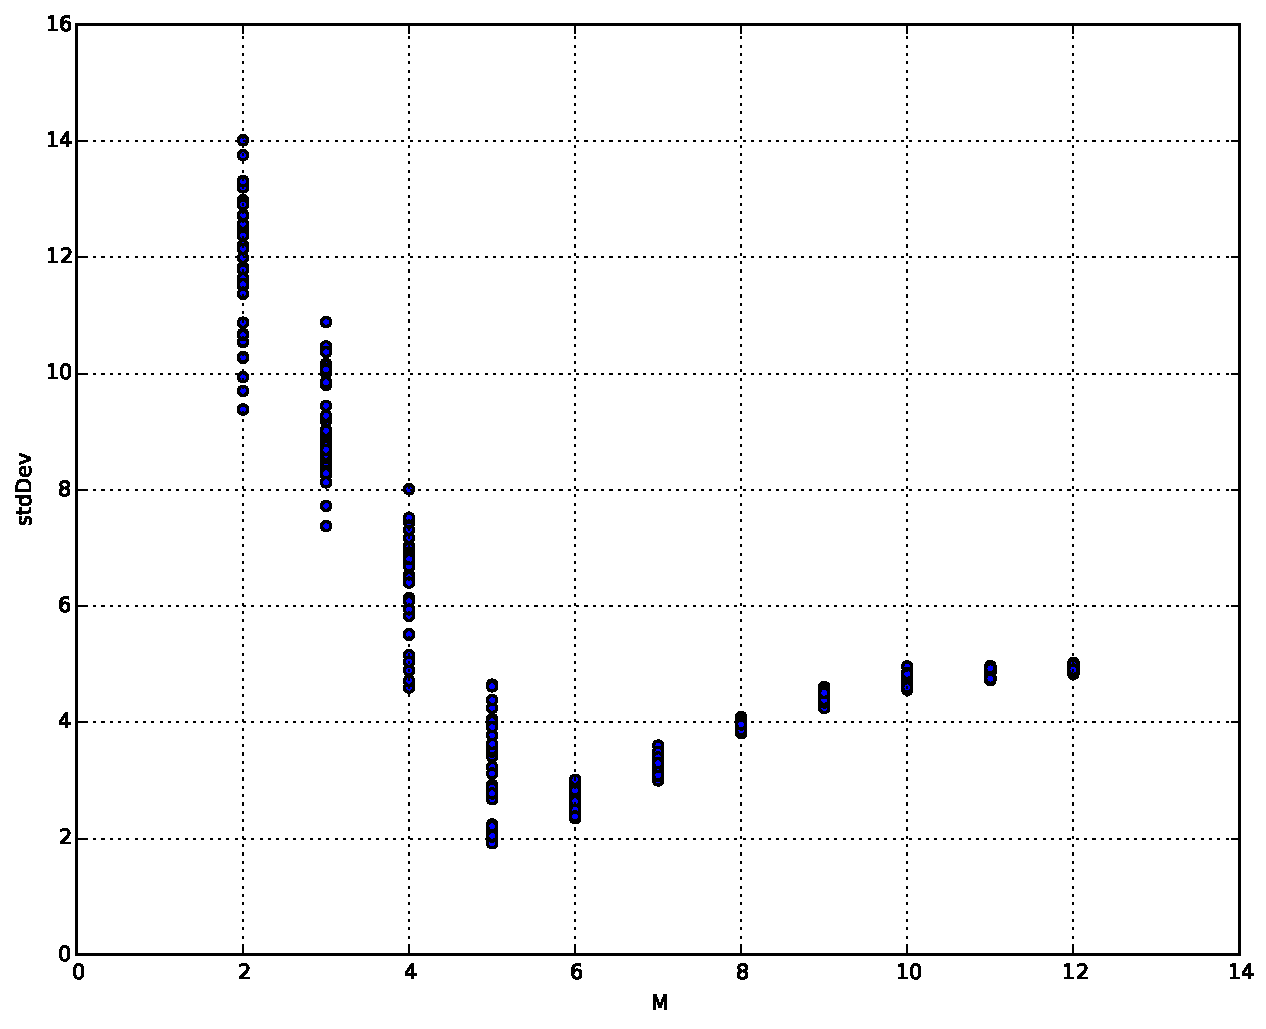
\includegraphics[scale=0.4]{images/minority/memory_to_stddev.pdf}
\caption{Plot of standard deviation of attendance for a model with 101 agents and 32 runs. In the axis memory (brain size) of agents}
\label{fig:memory to stddev}
\end{center}
\end{figure}

We can see that there is a minimum of the function somewhere between value $5$ and $6$ for memory.
Before this point standard deviation is definetly high with respect to the rest of the graph, and after the critical point it seems to converge to a fixed value.

It is already evident that there is a certain connection between the memory of agents and their ability to perform efficiently, intended as a efficient distribution of the resource they are competing for.
In this graph however $N$ is a fixed value, so let us see what happens when we start varying both parameters. 

\subsection{Phase Transition}
\label{subsec:phasetransition}

After further studies Savit, Manuca and Riolo \cite{savit1999adaptive} have noted that the macroscopic behaviour of the model is not characterized independently by the single parameters $M$ and $N$, but rather by the relation between the two.
They have discovered that a new control parameter $\alpha$, defined as $\alpha=\frac{2^M}{N}$, determines the volatility of the model.
Volatility is defined as a normalized variance:
\begin{displaymath}
\frac{\sigma^2}{N}
\end{displaymath}
The volatility depends only on the ratio between $2^M$ and $N$ and it does not get influenced by the source of information, meaning that it maintains it's characteristic behaviour in endogenous and exogenous games.

In Figure \ref{fig:normalized variance} volatility is plotted versus the control parameter $\alpha$.
The red line in the graph represents the volatility of a \textit{random-choice} model.
If we create a model where all the agents make random decision at every step the volatility that we obtain is:
\begin{displaymath}
\frac{\sigma^2}{N} = \frac{Np(1-p)}{N} = 0.5(1-0.5) = 0.25
\end{displaymath}
This is calculated assuming a binomial distribution of agent's actions with probability $p=0.5$.

\begin{figure}[h]
\begin{center}
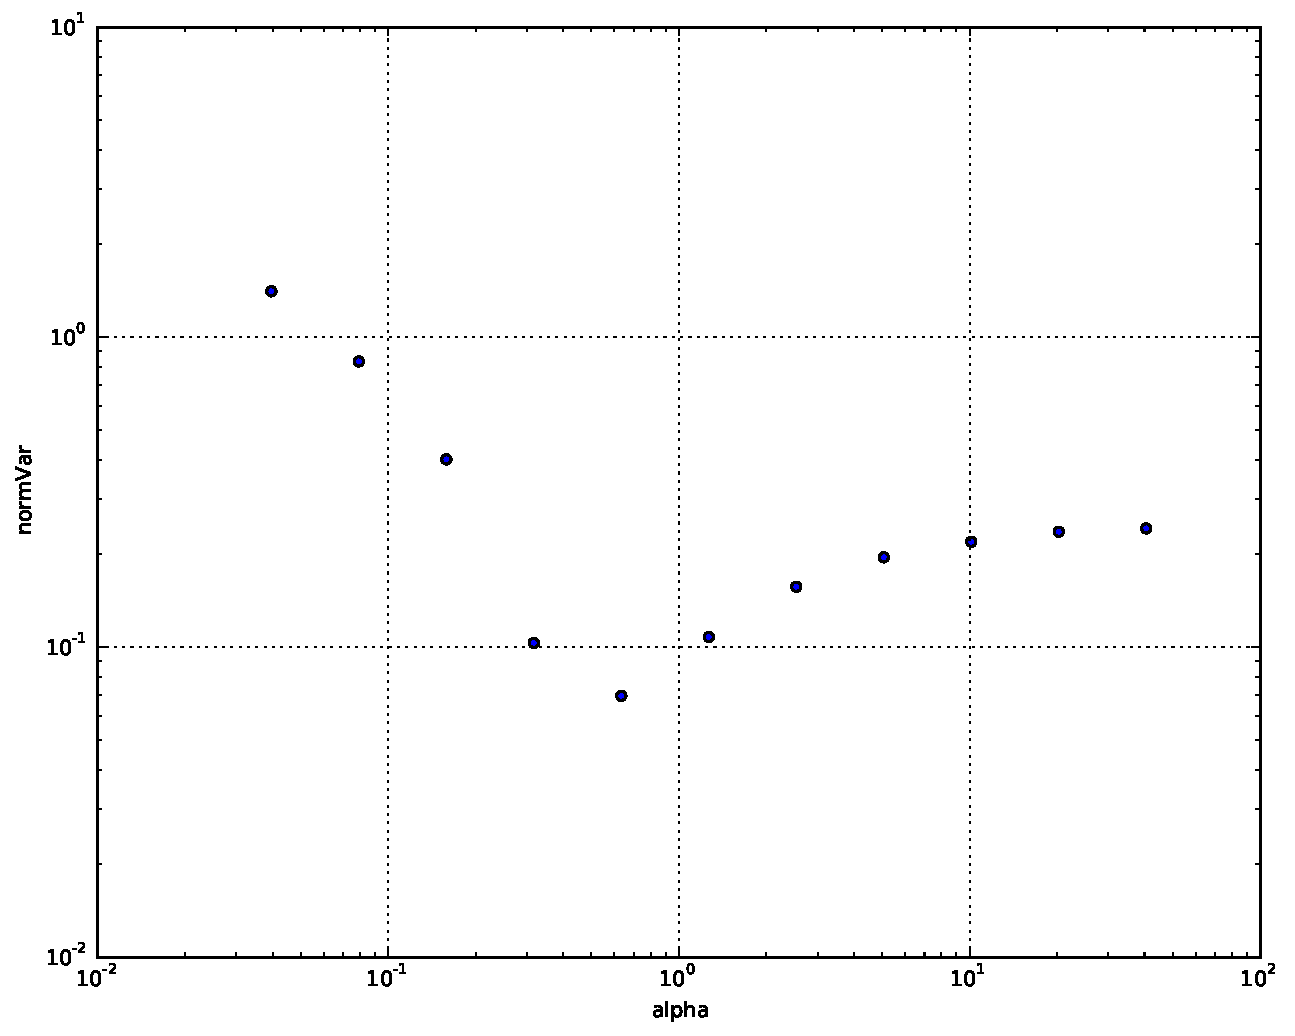
\includegraphics[scale=0.4]{images/minority/alpha_to_norm_var.pdf}
\caption{Plot of normalized variance versus control parameter $\alpha$}
\label{fig:normalized variance}
\end{center}
\end{figure}

Looking at the graph \ref{fig:normalized variance} we can see that for low values of our control parameter $\alpha$ agents perform worse than they would if only random decisions where made.
By incrementing the control parameter, either by raising the memory available or by removing certain quantities of agents from the model, the volatility pummels to it's minimum at the critical value of $\alpha$ ($\alpha_c$).
This critical value has been calculated in \cite{marsili2000exact} by Marsili \textit{et al.} and is approximated to $0.3347$ for $S=2$.
By incrementing further the control parameter the volatility starts incrementing again and converges to the random choice limit.

This behaviour can be observed if we look at the plots of attendance for models with different values of $\alpha$. In figures \ref{fig:attendance_m2}, \ref{fig:attendance_m5} and \ref{fig:attendance_m9} graphs of attendance can be seen for models consisting of $101$ agents but with varying memory size. Different brain sizes plotted here are $2$, $5$ and $9$, which gives us $\alpha$ values of $0.03960$, $0.3168316$ and $5.0693069$ respectively. For $\alpha$ bellow it's critical value we can see that the variance of the attendance is rather high, it becomes minimum for $M=5$.
Basic intuition would tell us that by further increasing the memory of the agents we can bring the volatility even lower, but the results show differently.
By increasing further the brain size agents start to have very different strategies and can no longer exploit the information present in the model, and end up acting like random agents. 
This can be seen in figure \ref{fig:attendance_m9} where the memory has been increased to $9$ and the volatility has returned to be higher than in the previous case of $M=5$.

\begin{figure}[h]
\begin{center}
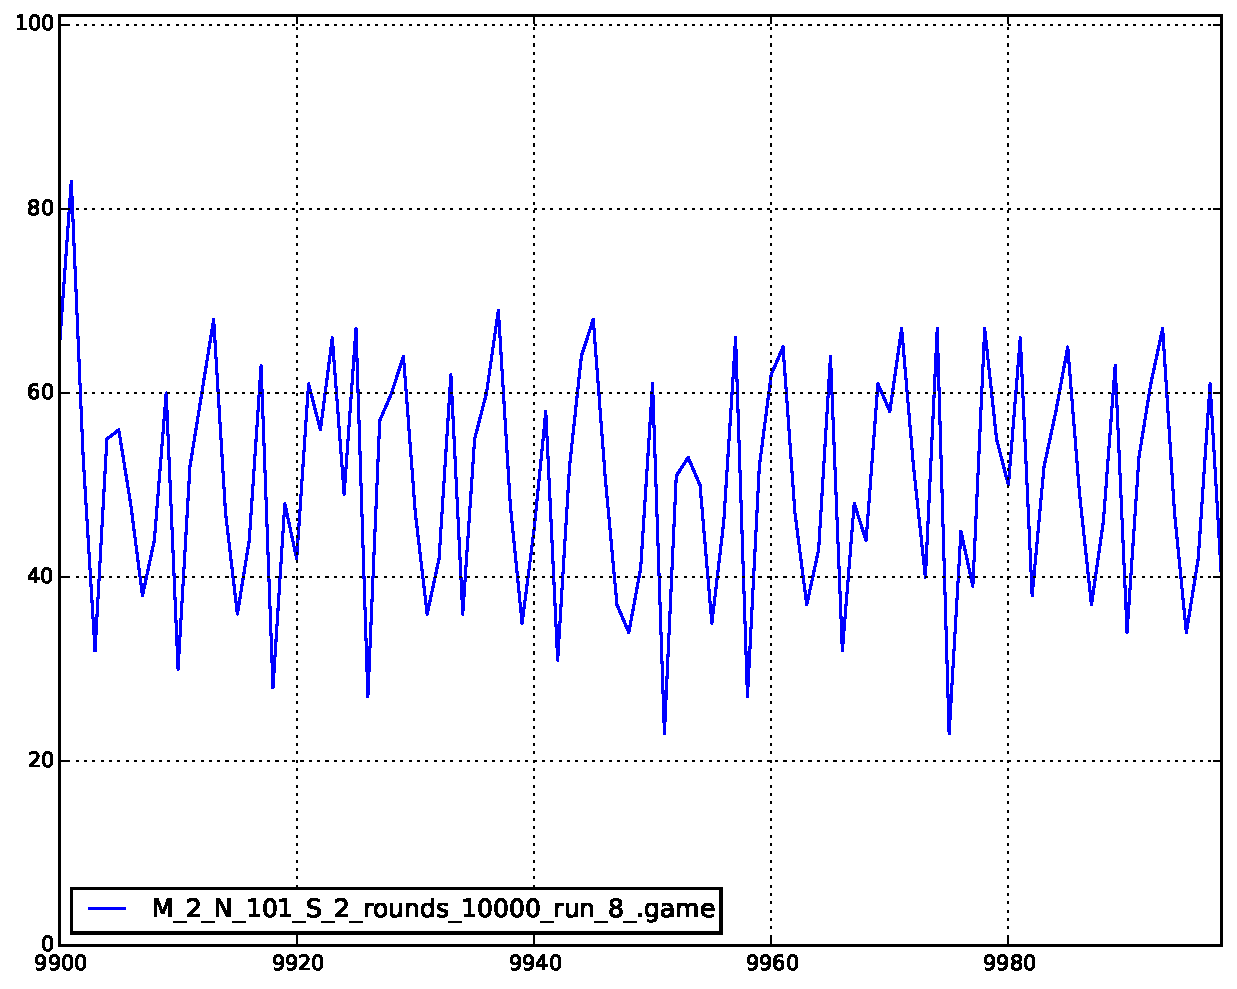
\includegraphics[scale=0.4]{images/minority/attendance_m2_n101.pdf}
\caption{Plot of attendance over time for a model with agents with $M=2$ and $N=101$}
\label{fig:attendance_m2}
\end{center}
\end{figure}

\begin{figure}[h]
\begin{center}
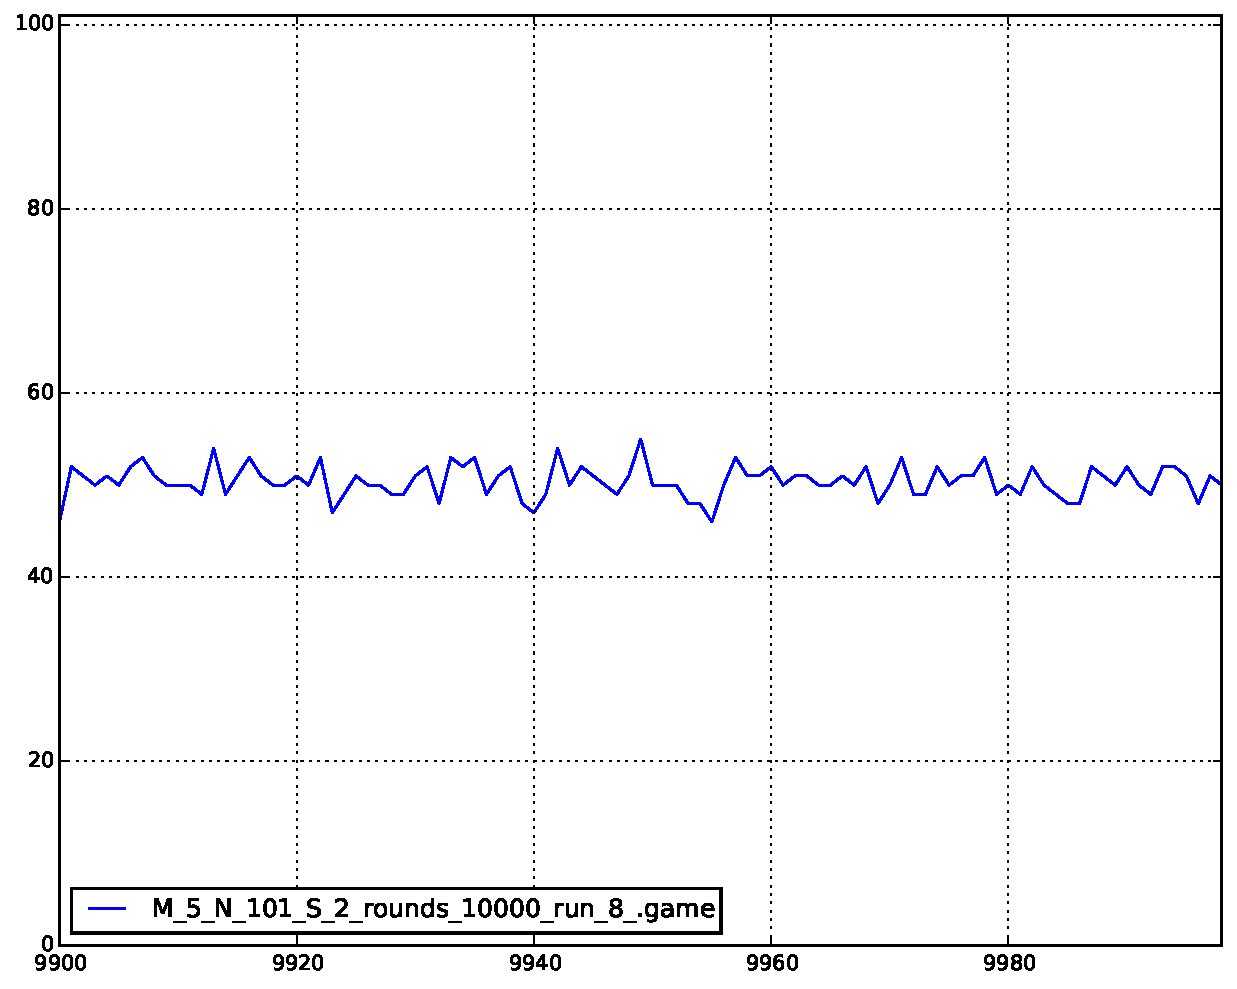
\includegraphics[scale=0.4]{images/minority/attendance_m5_n101.pdf}
\caption{Plot of attendance over time for a model with agents with $M=5$ and $N=101$}
\label{fig:attendance_m5}
\end{center}
\end{figure}

\begin{figure}[h]
\begin{center}
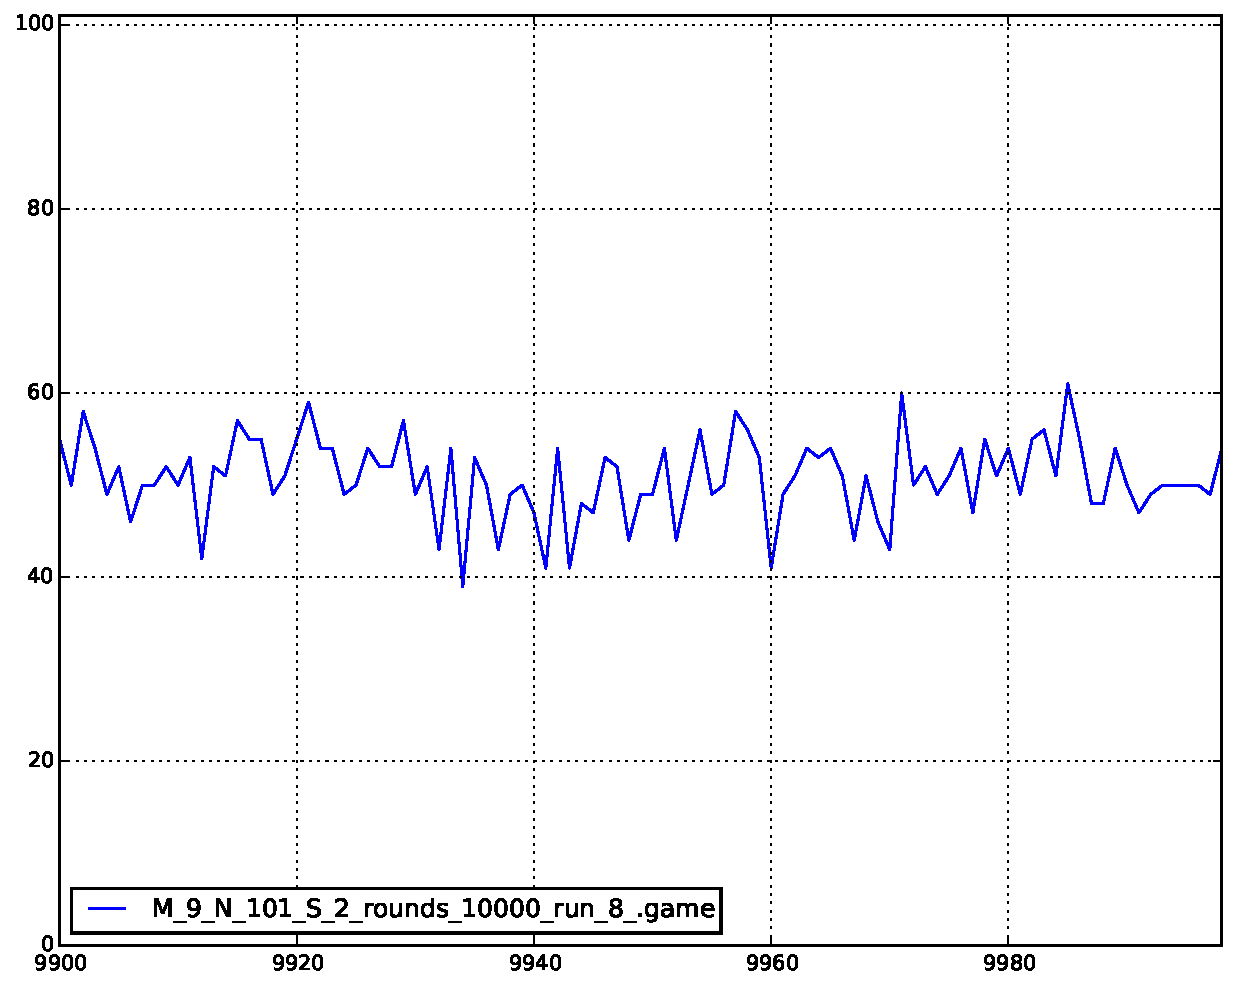
\includegraphics[scale=0.4]{images/minority/attendance_m9_n101.pdf}
\caption{Plot of attendance over time for a model with agents with $M=9$ and $N=101$}
\label{fig:attendance_m9}
\end{center}
\end{figure}

The $\alpha_c$ identifies a separation between two phases of minority games.
To characterize better the two phases let's look at the information available to agents in different phases.
We plot the probability of "1" being the winning choice given a certain history, $P(1|\mu)$ in figures \ref{fig:information_44} and \ref{fig:information_66}.
When the control parameter is below it's critical value $\alpha_c$ the probability of "1" being the winning side is equal to $0.5$ for all values of history $\mu$.
This shows the fact that there is no information to be extracted from the model for agents of that particular brain size, ie. all the outcomes seem to be random.
For reasons expressed, this phase is called \textit{unpredictable} phase or also \textit{symmetric} phase for the symmetry present in the probability mass function given a certain history.
If we look at the graph of probability given a certain history when the control parameter $\alpha$ is above it's critical value, given in figure \ref{fig:information_66}, we can see that there is information available to be exploited in this phase.
This phase hence is called \textit{asymmetric} or \textit{predictable}.
In this phase agents act better than when making random choices, and even though each agent acts in his self best interest we can say that a phenomenon of cooperation emerges as the agents are able to distribute themselves on both sides with rather small variance.
Note that even in the asymmetric phase model retains it's \textit{negative-sum-game} nature and majority of the agents continue to lose, however the number of losing agents is brought to it's minimum.


% probability of 1 given a history
\begin{figure}[h]
\begin{center}
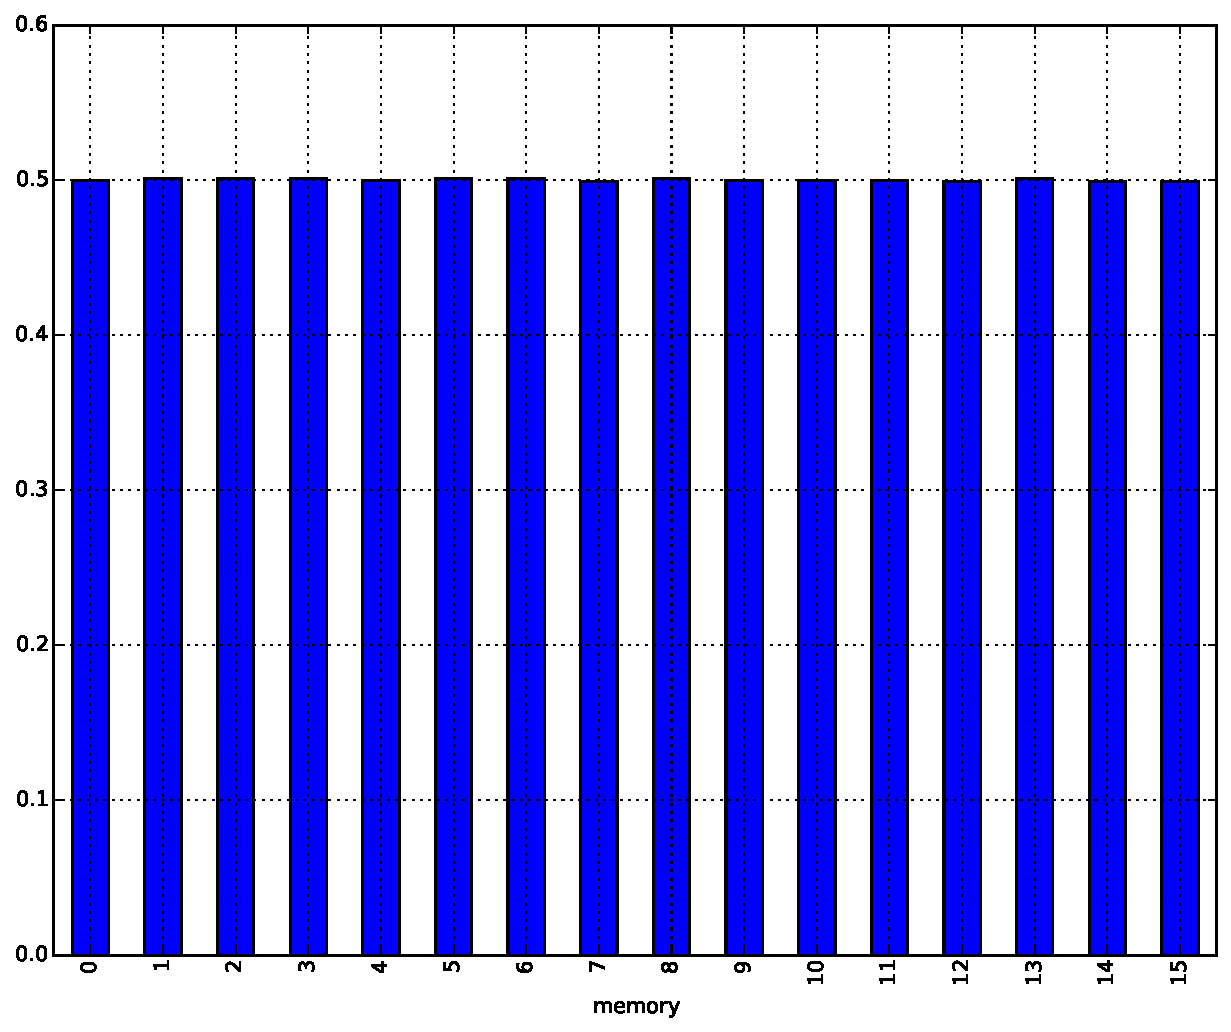
\includegraphics[scale=0.4]{images/minority/information_probability_m4_a4.pdf}
\caption{Plot of $P(1|\mu)$ versus $\mu$ using a sliding window of length $4$ on a model where agents have $M=4$}
\label{fig:information_44}
\end{center}
\end{figure}

\begin{figure}[h]
\begin{center}
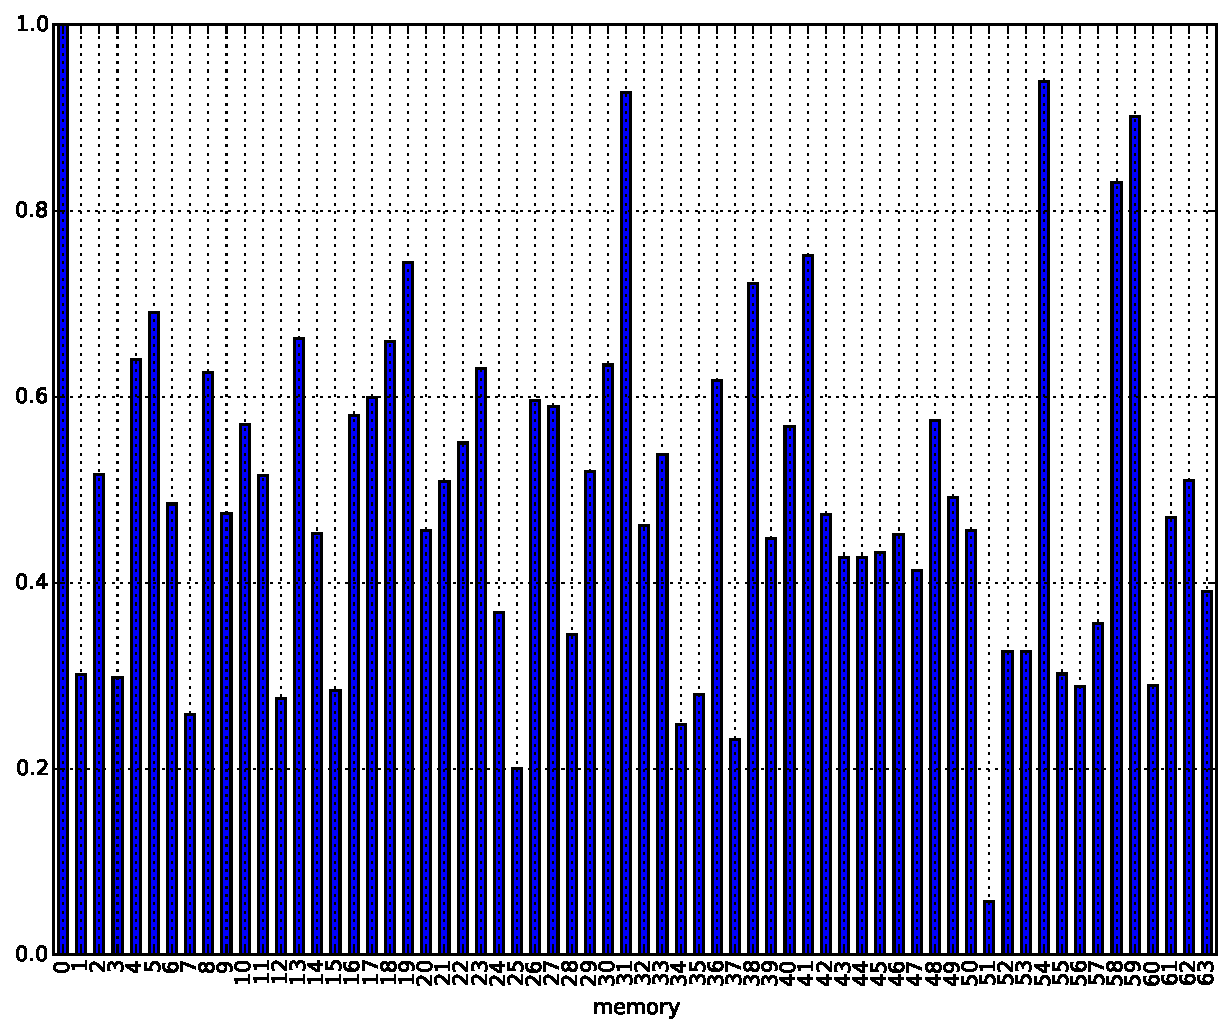
\includegraphics[scale=0.4]{images/minority/information_probability_m6_a6.pdf}
\caption{Plot of $P(1|\mu)$ versus $\mu$ using a sliding window of length $6$ on a model where agents have $M=6$}
\label{fig:information_66}
\end{center}
\end{figure}

It is important to note that the information is present within the model even in the symmetric phase, but the agents don't have the capabilities to exploit that information.
In fact, if we introduce an agent with $M$ greater that those of agents already in the \textit{symmetric} phase we can expect that he will be able to exploit his advantage of greater memory.
The information present in the model for an agent with larger brain size can be seen in figure \ref{fig:information_35} that plots the probability that "1" will be the minority size versus the possible history.

\begin{figure}[h]
\begin{center}
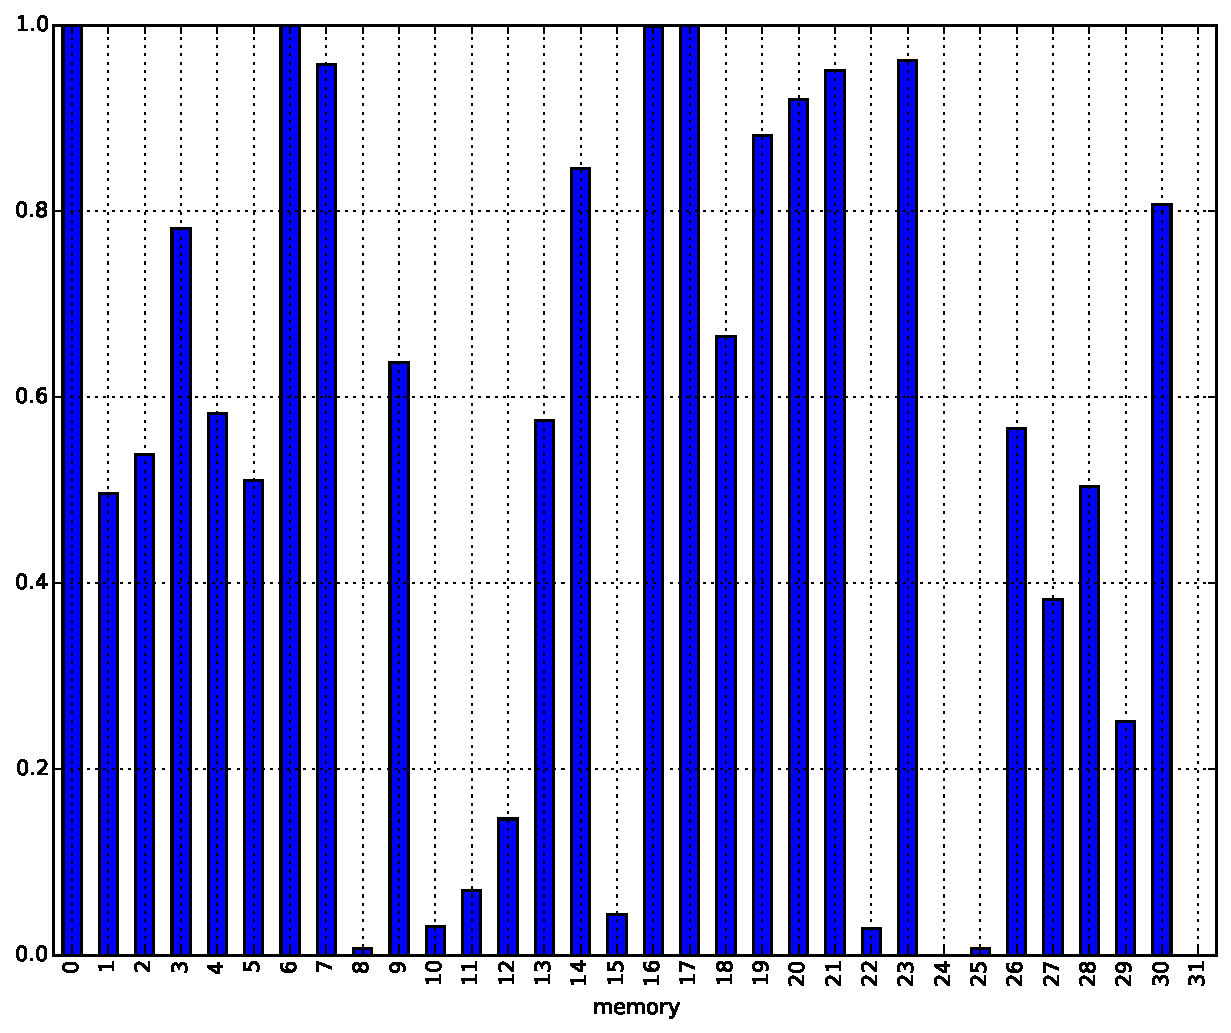
\includegraphics[scale=0.4]{images/minority/information_probability_m3_a5.pdf}
\caption{Plot of $P(1|\mu)$ versus $\mu$ using a sliding window of length $5$ on a model where agents have $M=3$}
\label{fig:information_35}
\end{center}
\end{figure}

\subsection{Crowds and anti-crowds}
\label{subsec:crowds}

The nature of \textit{symmetric} phase brings about the phenomenon of the formation of crowds and anti-crowds.
When we find ourselves in the symmetric phase the $\alpha$ is below it's critical level, meaning that $2^M$ is roughly one order of magnitude smaller than $N$.
The consequence is that the number of available strategies $2^{2^M}$ is low when compared to the number of agents, hence probability of different agents having the same strategies is higher than in the \textit{asymmetric} phase.
Another way to explain the phenomenon is to say that when $M$ is low agents are able to efficiently elaborate the information, however since the information is short many agents will come to the same predictions, and behave in the same fashion.

The phenomenon of crowds and anti-crowds thus happens in symmetric phase and when it occurs most of the agents behave in the same way, giving rise to high volatility.
If number of agents is large and the number of available strategies is small, it is more opportune to make decisions randomly rather than use deterministic strategies.

\section{Variations for financial markets}
\label{minority:variations}

The basic minority games introduce a very simple model for the financial markets, however there are certain modification to be done before we can start comparing it to a real market.
Let us assume that the action "1" stands for "buy" and action "0" stands for sell.
Attendance can now be seen as a number of agents that participate in the market as buyers, while $N-A(t)$ is the number of sellers.
The quantity $A(t)-\frac{N}{2}$ is the excess demand in the market.
So if that quantity is positive most of the agents involved are buyers and it is profitable at that moment to sell, and viceversa.
This is an economical point of view to the basic mechanism of minority games.
The payoff that is given to agents at each round, introduced in \cite{challet2001stylized}, is defined as
\begin{displaymath}
g_i(t)=a_i(A(t) - \frac{N}{2})
\end{displaymath}
This captures the fact that the agent on the minority side are awarded proportionally to their investment.

To model the prices Challet \textit{et al.} have used this price dynamic in their original paper:
\begin{displaymath}
\log p(t+1) = \log p(t) + \frac{A(t)}{\lambda}
\end{displaymath}
where $\lambda$ is related to the market depth.
By setting the parameter $\lambda$ to a low value we obtain a market with higher fluctuations, with the opposite giving us a more smooth price transitions.
The fluctuations happen in the same fashion with different values of $\lambda$, what changes is the variance but the qualitative properties remain the same.

The most important modification of the basic model when trying to simulate financial markets is the introduction of two types of agents, \textit{producers} and \textit{speculators} that interpret different approaches to the real market.

\subsection{Producers}

Producers, per definition, contribute to the market always following a predetermined behaviour.
They model the agents that produce goods and services, and as such participate in the market at all times.
Since their scope is not to speculate on other agents behaviour but to use market to sell their goods/services and buy other goods/services needed, they have a deterministic behaviour, acting always in the same fashion for same values of $\mu(t)$.
Inside the model of the market they create information that is then exploited by speculators.

Producers are modelled starting from our basic model and giving them only one strategy.
Other changes to this agent are not necessary as all the basic definitions still hold true.
Participation is already obligatory in the basic model and having only one strategy makes the behaviour of the producers deterministic.

\subsection{Speculators}

Speculators on the other hand do not produce goods or services, but use the market to exploit the information injected in the model by the producers to gain profit.
Two main differences between speculators and producers are that speculators have adaptive behaviour and that they can choose not to participate in the market if they find it unprofitable.

In order to model adaptive behaviour $S$ strategies are given to each speculator, drawn randomly from $2^{2^M}$, from which he can choose.
As for the ability to abstain from the market in unfavourable conditions we add yet another strategy, called \textit{0-strategy} that tells the speculator not to interact with the market at chosen time.

At each round the speculator chooses the best strategy by picking the one with the highest virtual score, calculated with:
\begin{displaymath}
U_{i,s}(t+1) = U_{i,s}(t) - [(2a_{i,s}^{\mu(t)}(t+1)-1)(A(t)-\frac{N}{2}) ] + \epsilon\delta_{s_i(t),0}
\end{displaymath}

with

\begin{displaymath}
\delta_{s_i(t),0} =
  \begin{cases}
    1       & \quad \text{if } i = 0 \quad \text{ie. zero strategy}\\
    0       & \quad \text{if } i \neq 0 \quad \text{ie. others strategies}\\
  \end{cases}
\end{displaymath}

The first part of the formula is the same as the virtual score calculation for the basic model, ie. a strategy is awarded points if it correctly predicts the minority side.
The second part models the virtual score of the zero strategy that get incremented at every step by $\epsilon$.
This new parameter models the interest rate for the speculators, making them active participants in the market with only the strategies that can guarantee a profit over time that is larger than $\epsilon t$, with t the number of rounds thus far.
Note that all the considerations above are made with the assumption that $\epsilon$ is positive, in fact if we set $\epsilon$ to be infinitely negative value speculators act as agents in the basic model.

\subsection{Market ecology and crash simulation}

To simulate markets a minority game is defined with a certain number of producer and speculator agents.
The market is characterized by the relationship between these two quantities.
As producers behave in a deterministic fashion we can say that they introduce information inside the model that can be exploited by the speculators.
Speculators on the other hand participate when they have a strategy that can consistently outperform the  producers, ie. if the virtual score of the strategy is larger than $\epsilon t$, where $t$ is the time and $\epsilon$ models the interest rate.

If the number of producers is sufficiently high and greater than the number of speculators, than a majority of speculators will be always active as the information introduced by producers is high as well as the possibility to have a strategy that can use that information.
On the other hand when the number of speculators is higher than the number of producers, a majority of speculators will not participate in the market.

The dynamic when a great quantity of speculators is present, compared to the number of producers causes high volatility in the market.
In the beginning the speculators participate in the market, but after certain period $t_1$ the zero-strategy starts to have higher virtual score than the rest of strategies, causing speculators to abstain.
After $t_1$ then the majority of agents involved are producers that introduce information in the model, so after a second interval at time $t_2$ certain number of speculators start acting inside the market again and reduce the information available.

\begin{figure}[h!]
\begin{center}
	\begin{subfigure}[b]{0.5\textwidth}
	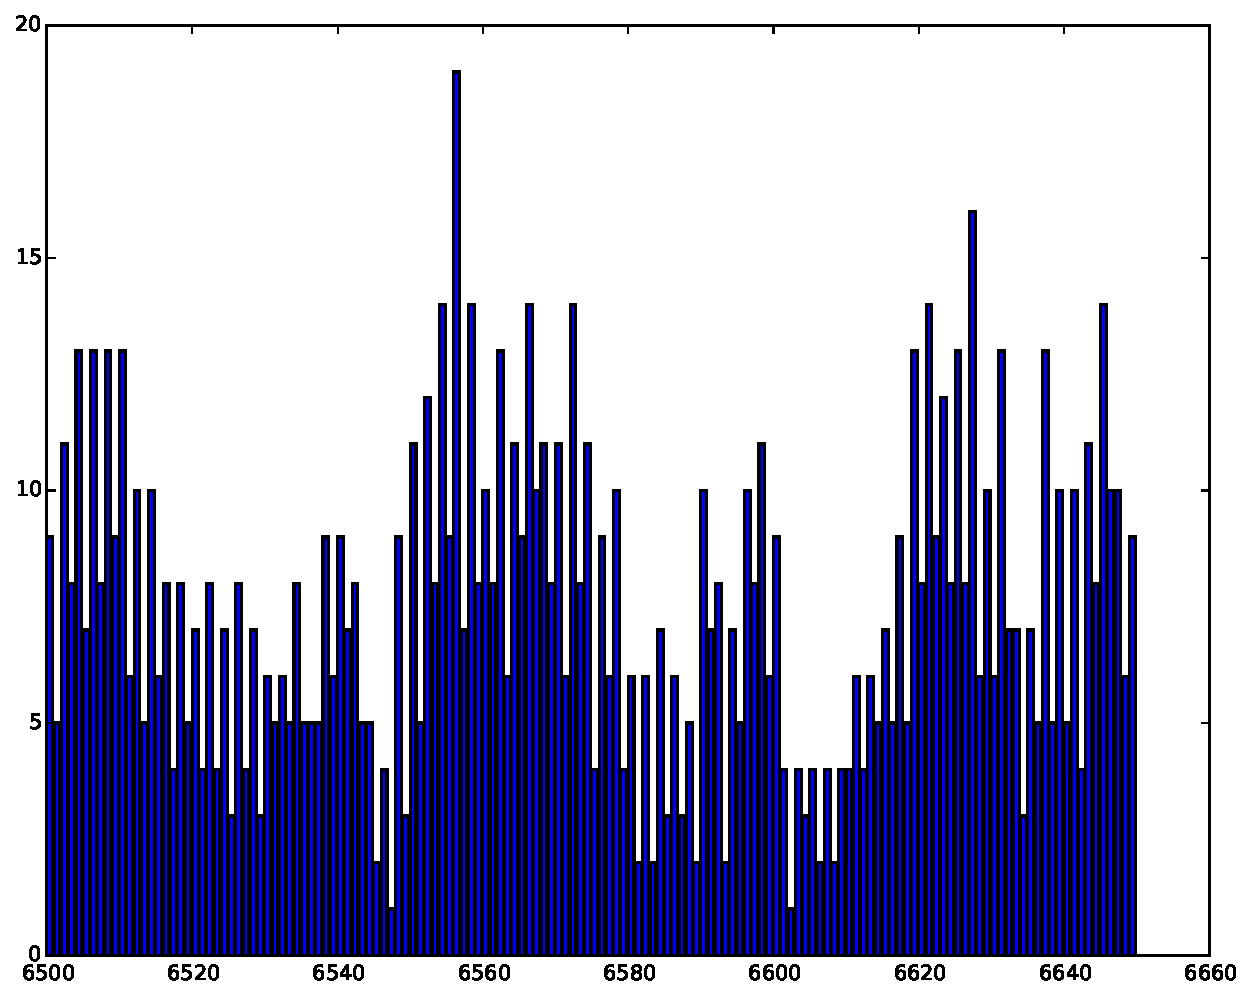
\includegraphics[scale=0.4]{images/minority/active_speculators_np10_ns300.pdf}
	\caption{Number of active speculators in a game with 10 producers and 300 speculators}
	\end{subfigure}
	\begin{subfigure}[b]{0.5\textwidth}
	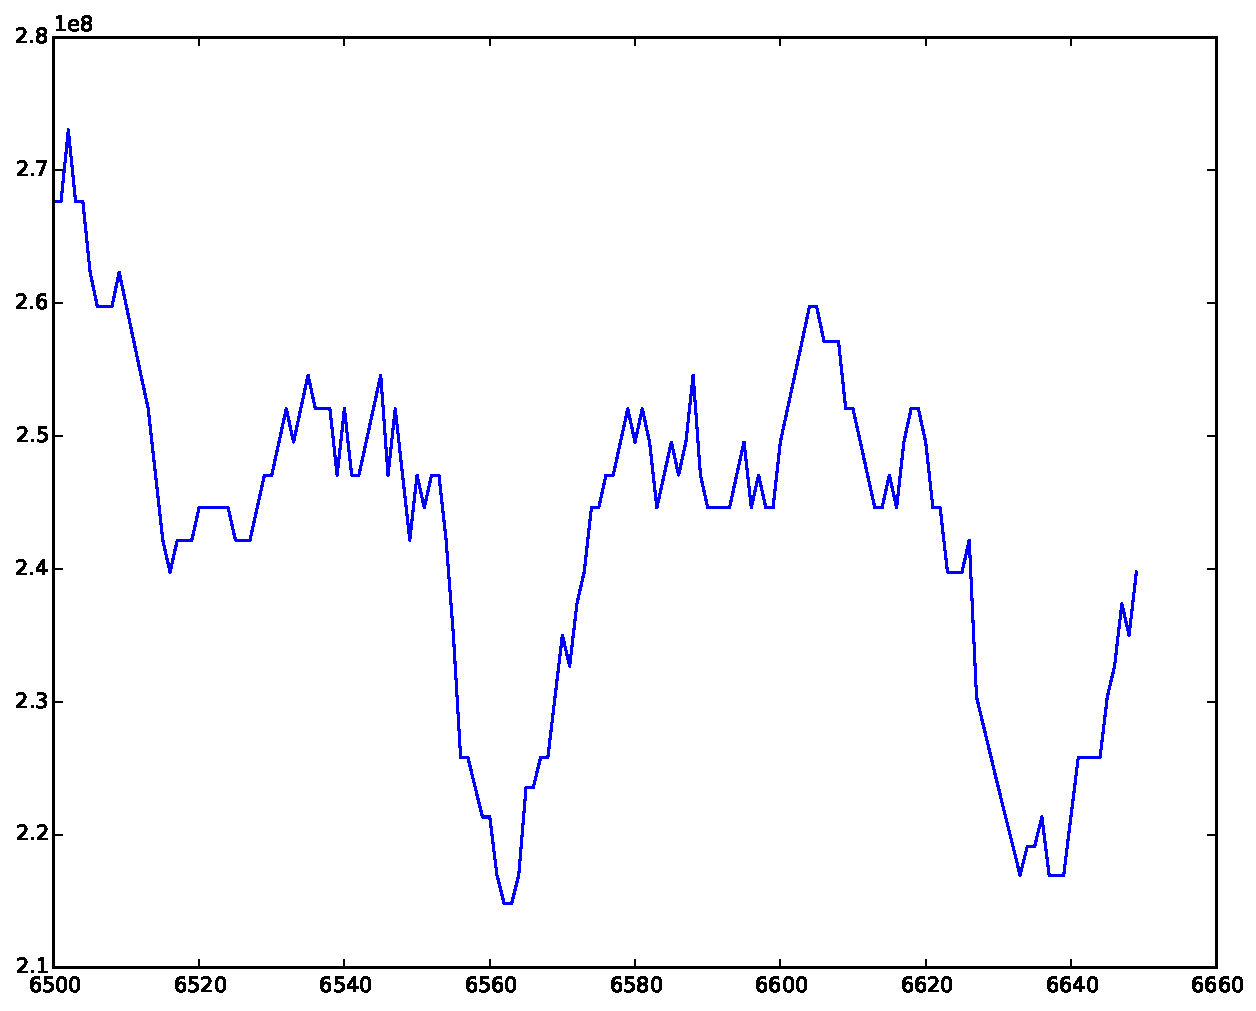
\includegraphics[scale=0.4]{images/minority/market_price_np10_ns300.pdf}
	\caption{Market price for the same game in the same interval}
	\end{subfigure}
\caption{Active speculators and market price}
\label{fig:active speculators}
\end{center}
\end{figure}

This behaviour of speculators causes the price to fluctuate and can cause crashes and spikes inside the market.
An example is shown in figure \ref{fig:active speculators}, where in \ref{fig:active speculators}.(a) we can see the number of active speculators and in \ref{fig:active speculators}.(b) the market price generated with the mechanism described in \ref{minority:variations},
We can see that the sudden participation of a great number of speculators in the model can cause crashes. 

Further step in simulating financial markets with minority games would be by introducing the capital property of the agents.
It can easily be simulated like the score the agents just like the virtual scores of strategies are modelled.
Instead of using the $\sign$ function to discriminate between winning and losing agents, we can use $g_i(t)$ defined as

\begin{displaymath}
g_i(t)=a_i(t)(A(t) - \frac{N}{2})
\end{displaymath}

and adding this value to the total \textit{capital} of the agent.
By removing the $\sign$ function, the agents are earn/lose proportionally to the volatility present in the market. 
For example, if more agents decide to sell, while a low number of agents decide to buy, the buyers can dictate the price as the supply is enormous and the demand low.
This translates to a higher profits proportional to the difference $[A(t)-\frac{N}{2}]$.
These sort of modifications were not simulated in this thesis as the focus was on the quantity of information and the topology of the network between agents, but it has been taken in consideration while studying the possible application of the results to financial markets. 

\section{Vicinity information}
\label{minority:vicinity}

The basic minority games, as well as all the variations presented in this chapter, do not allow for direct communication between agents.
The exchange of information is done by passing to each agent the global history.

In this thesis we have decided to study how does the basic model of minority games change when a network structure is added.
The agents inside the model become the nodes of the network and the edges between different nodes become the connections for information exchange.

Starting from the observations done in subsection \ref{subsec:phasetransition} certain assumptions are justified and have been proven through computational simulation.
If we want to obtain a more efficient model in distributing limited resources the best way to intervene is to minimize the volatility.
By looking at the Figure \ref{fig:normalized variance} the easiest way to accomplish this is by modifying the $\alpha$ parameter in order to bring the model in the cooperative regime.
For example, when the $\alpha$ is below the critical value $\alpha_c$ two possibilities are open, whether increase the memory of the agents or reduce the total number of agents.
The second option is less preferable in the majority of systems if not all, as in most systems once the agents are allowed to participate it can prove difficult to reduce their number (think of drivers in traffic).
This leaves us with the first option, the one where new information is added to the model and the memory of agents is expanded.
The easiest way would be to just increase the memory without differentiating the information given to the agents.
However, our intuition, later proved by the experimental results, has suggested that a differentiation of information could improve the efficiency of the model.
The new information added for each agents are the results of minority games done in the vicinity of the said agent.
The network theory and the results expected by this new information introduced in the model are described in Chapter \ref{chapter:vicinity}.


Equivalent way of thinking can be applied to the case when $\alpha$ is much higher than it's critical value, and brings the model to the \textit{random-choice} volatility levels.
In this case the total information in the model need to be reduced in order to lower the volatility.

To close this chapter we return to the initial inspiration for the minority games to explain our decision to include vicinity information.
In the El Farol bar problem each person decides whether to attend the bar or not based on the past attendances.
If we would like to improve the efficiency of the El Farol bar participation when the model is in the symmetric phase, the obvious choice as explained in this section is to give greater brain size to people, ie. let them remember more in the past, so instead of remembering last 3 Thursdays a person now recalls last 5 or 6 Thursdays.
But if we want to represent this problem realistically it is impossible to discard the fact that people do talk to each other, and allow for the information to flow through smaller groups inside the community.
This simple truth has brought us to include inside the model the vicinity information and study how it affects the efficiency of the games, whatever their application may be.
% Neighbourhood influence on the model
\chapter{Neighbourhood and other information in the model}
% Results and real world applications
\chapter{Initial results with different topologies}
\label{chapter:results}

In this chapter we present the results obtained through computational simulation of the minority games that include vicinity and are characterized by different network structures.

In Section \ref{sec:spacetime} we describe the role of information in competitive systems simulated with minority games in more detail, as it has already been mentioned in other parts of this work.
In Sections \ref{sec:fixed} and \ref{sec:hierarchical} we present the results for each network topology separately based on different parameters of the models.
After that in Section \ref{sec:confrontation} we confront different topologies to each other and explain the results.
Final two Sections, \ref{sec:spacetime2} and \ref{sec:final}, talk about the different role of information in the light of the results and conclude with some thoughts on competitive systems with limited resources. 

\section{Information in space and time}
\label{sec:spacetime}

From the initial studies of the competitive systems based on minority games we have seen that these models have two different phases of operation.
The separation of the two phases is defined by the relationship between the quantity of the information each agent can process and the number of agents, just as explained in subsection \ref{subsec:phasetransition} where $\alpha$ control parameter is defined.
The efficiency of the model, measured in the capacity to distribute the resources between agents, is best around the critical value of $\alpha$.
From this observation we can easily deduce that in order to optimize any kind of competitive system with similar mechanics we need to tinker with the $\alpha$ parameter to bring the volatility to its minimum.
Since $\alpha$ is defined as $\frac{2^M}{N}$ we are presented with a choice of either modifying the memory of the agents, their number, or both values at the same time.
Two important facts to note here and that have already been mentioned separately in previous chapters are: 
\begin{itemize}
\item In many systems to increase or decrease the number of agents involved is simply not realistic, as this could prove an inefficient and discriminatory politic. Think of a navigation system for vehicles or data packets. Should we remove or add more drivers/packets in order to optimize the system? Adding new elements to the model would only optimize the macroscopic behaviour of the system, while the performance of the initial agents present in model would not improve, it could actually worsen. On the other hand removing elements from the model would cause discrimination between who is allowed to participate and use the limited resource. Thus for the purpose of this thesis we have worked with a fixed number of agents inside our models and have focused on modifying the second parameter $M$, the memory of the agents
\item Even as we bring the volatility to its minimum through parameter modification it still remains a \textit{negative-sum-game}. The optimization consist in making the number of losing agents as low as possible, but it will always remain greater that the number of winning agents.
\end{itemize}

\begin{figure}[h]
\begin{center}
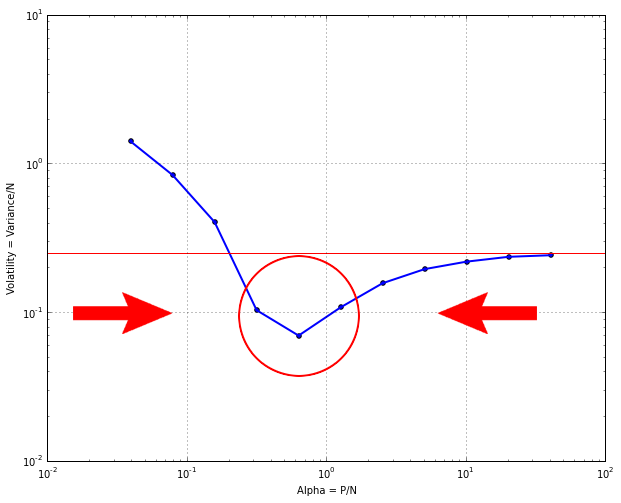
\includegraphics[scale=0.4]{images/results/alpha_to_norm_var2.png}
\caption{Plot of normalized variance versus control parameter $\alpha$ for a basic minority game}
\label{fig:normalized variance spacetime}
\end{center}
\end{figure}

We are left with tinkering with the quantity of information available to agents in order to minimize the volatility that is well defined and can be calculated with enough simulations from other parameters of the model, mainly the number of agents, but others like the number of strategies $S$ can influence it.
In Figure \ref{fig:normalized variance spacetime}, the example taken from subsection \ref{subsec:phasetransition}, we have pointed out the cases when the increase or the decrease of information is necessary.

Two more observations are needed before we dive into the analysis of the experimental results.
Foremost, not only can we optimize the system by changing the quantity of the information available to single agents, we can also work on the quality of that information. Of course the information added to the model has to be relevant to the system, but as we have seen from our results some scenarios are more desirable.
Let us assume $\mu(t) = (i_1,i_2,\ldots,i_m)$ the information available to the agent, represented as $m$ bits.
In classical minority games all the information is generated by the single global minority games, but nothing stops us from differentiating the information available.
Driven by the basic intuition that the differentiation of information is preferable and inspired by the fact that real world examples of the systems simulated offer the possibility to communicate, we have decided to optimize the model by adding the information from the community of the agent.
In this way we make a distinction between the global information based only on time, and the local community information based also on time but with a spatial component defined as the topology of the network.
This approach is realistically most probable, especially in the case when we have to increase the quantity of information, since temporally more distant data could not be available or due to the possible changing topology of the model (in real world agents participate for certain periods of time, until their needs are met) that renders temporally more distant data less reliable.
This intuition has brought us to include the locally available information and to test different network topologies described in \ref{chapter:vicinity}.

Second observation before diving into the experimental results is that when we have said that we only modify the brain size of agents and not the total number of agents, we have oversimplified our model.
Actually by adding local information and dividing the set of agents in communities, we are in a indirect way modifying the volatility of the model by creating smaller instances of minority games that bring the control parameter $\alpha$ closer to its critical value.
Of course the total number of agents remains the same and they are always present in the global minority game.

\section{Fixed community structures results}
\label{sec:fixed}

By fixed community structures we intend the fixed one-dimensional isolated communities described in Section \ref{sec:fixed communities}, sliding window one-dimensional communities defined in subsection \ref{subsec:sliding} and von Neumann neighbourhood described in Section \ref{sec:von neumann}.

In this section and the next one we use a new parameter $\beta$ to represent the relationship between the degree of each node to the number of total nodes, ie. the number of neighbouring agents versus the number of total agents.

\begin{displaymath}
\beta = \frac{d}{N}
\end{displaymath}

where $d$ is the mean degree of nodes in the network.

\subsection{Fixed one-dimensional communities}

The most simple topology is that of completely isolated local communities, also called patch neighbourhood. It can be seen in Figure \ref{fig:patch vicinity partial} that for various values of $\alpha$, different values of $\beta$ are optimal.

The data for the first two curves equivalent to models with information length $4$ and information length $6$ are shown in Tables \ref{table:fixed m4} and \ref{table:fixed m6}.
First three rows of each table has been highlighted and tells us what the minimum $\beta$ should be when planning a competitive system with certain $\alpha$ in order to minimize the loses.
So we can see that for $\alpha=0.03990025$ our best option is to keep our $\beta$ around $0.05$, that is divide the whole population in around 20 communities in case of patch neighbourhoods, or make the mean degree of nodes $5\%$ of the total number of nodes in other types of networks.
But $\alpha=0.03990025$ is still low to bring a system in a bit more efficient regime, so we look at the second curve from Figure \ref{fig:patch vicinity partial} where $\alpha=0.159601$.
For that value of $\alpha$ our best option is to keep our $\beta$ in the interval $[0.2,0.35]$, ie. divide the total number of agents in $3$ or $4$ big communities.

For successive network topologies we will only bring forth tables with best results, which here have been presented entirely.

\begin{figure}[h!]
\begin{center}
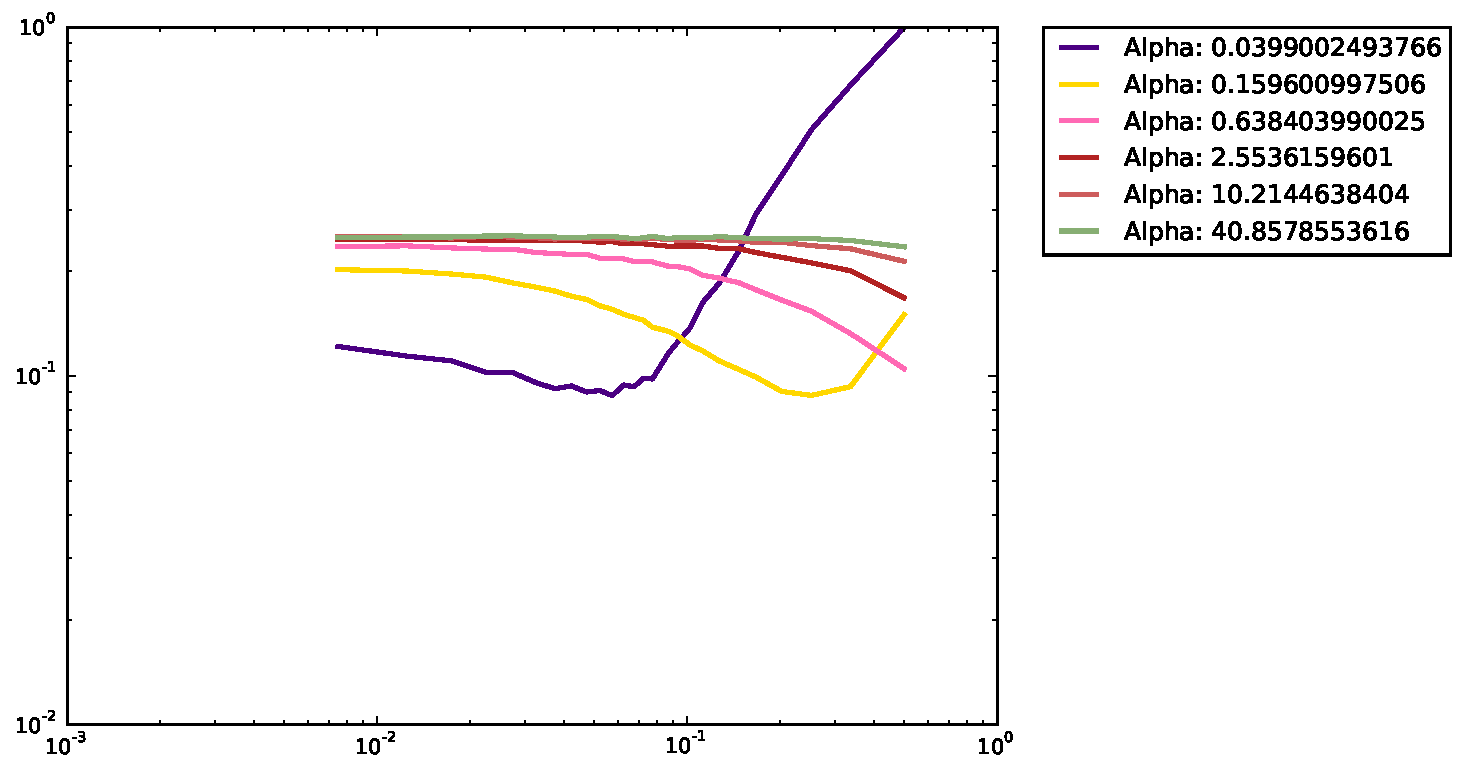
\includegraphics[scale=0.4]{images/results/vicinity_patch_n401_rounds10000_partial.pdf}
\caption{Plot of normalized variance versus control parameter $\beta$ for various values of $\alpha$  for fixed one-dimensional communities}
\label{fig:patch vicinity partial}
\end{center}
\end{figure}

\begin{table}
\tiny
\centering
\resizebox{\columnwidth}{!}{%
\begin{tabular}{lllllll}
\toprule
neighs &  M &    N &       alpha &         beta & meanNormVar &       var \\
\midrule
\rowcolor{Goldenrod}
    23 &  4 &  401 &  0.03990025 &   0.05735661 &  0.08778602 &  35.20219 \\
\rowcolor{Goldenrod}
    19 &  4 &  401 &  0.03990025 &   0.04738155 &   0.0899272 &  36.06081 \\
\rowcolor{Goldenrod}
    21 &  4 &  401 &  0.03990025 &   0.05236908 &  0.09083007 &  36.42286 \\
    15 &  4 &  401 &  0.03990025 &   0.03740648 &  0.09194704 &  36.87076 \\
    27 &  4 &  401 &  0.03990025 &   0.06733167 &  0.09309645 &  37.33168 \\
    17 &  4 &  401 &  0.03990025 &   0.04239401 &  0.09357988 &  37.52553 \\
    25 &  4 &  401 &  0.03990025 &   0.06234414 &   0.0941925 &  37.77119 \\
    13 &  4 &  401 &  0.03990025 &   0.03241895 &  0.09577665 &  38.40644 \\
    31 &  4 &  401 &  0.03990025 &   0.07730673 &  0.09799674 &  39.29669 \\
    29 &  4 &  401 &  0.03990025 &    0.0723192 &  0.09831647 &  39.42491 \\
    11 &  4 &  401 &  0.03990025 &   0.02743142 &   0.1021554 &  40.96432 \\
     9 &  4 &  401 &  0.03990025 &   0.02244389 &    0.102481 &  41.09487 \\
     7 &  4 &  401 &  0.03990025 &   0.01745636 &   0.1104009 &  44.27077 \\
     5 &  4 &  401 &  0.03990025 &   0.01246883 &   0.1139728 &  45.70309 \\
    35 &  4 &  401 &  0.03990025 &    0.0872818 &   0.1165516 &   46.7372 \\
     3 &  4 &  401 &  0.03990025 &  0.007481297 &   0.1214733 &   48.7108 \\
    37 &  4 &  401 &  0.03990025 &   0.09226933 &   0.1236184 &  49.57097 \\
    41 &  4 &  401 &  0.03990025 &    0.1022444 &   0.1373252 &  55.06739 \\
    45 &  4 &  401 &  0.03990025 &    0.1122195 &   0.1622121 &  65.04706 \\
    51 &  4 &  401 &  0.03990025 &     0.127182 &   0.1847199 &  74.07266 \\
    59 &  4 &  401 &  0.03990025 &    0.1471322 &   0.2288271 &  91.75965 \\
    67 &  4 &  401 &  0.03990025 &    0.1670823 &   0.2921831 &  117.1654 \\
    81 &  4 &  401 &  0.03990025 &     0.201995 &    0.375436 &  150.5499 \\
   101 &  4 &  401 &  0.03990025 &    0.2518703 &   0.5081641 &  203.7738 \\
   135 &  4 &  401 &  0.03990025 &    0.3366584 &   0.6818775 &  273.4329 \\
   201 &  4 &  401 &  0.03990025 &    0.5012469 &   0.9980141 &  400.2037 \\
\bottomrule
\end{tabular}%
}
\caption{Table of a model with $M=4$, with 2 bits dedicated to global game and 2 bits to local community information}
\label{table:fixed m4}
\end{table}

\begin{table}
\tiny
\centering
\resizebox{\columnwidth}{!}{%
\begin{tabular}{lllllll}
\toprule
neighs &  M &    N &     alpha &         beta & meanNormVar &       var \\
\midrule
\rowcolor{Goldenrod}
   101 &  6 &  401 &  0.159601 &    0.2518703 &  0.08792742 &  35.25889 \\
\rowcolor{Goldenrod}
    81 &  6 &  401 &  0.159601 &     0.201995 &  0.09028853 &   36.2057 \\
\rowcolor{Goldenrod}
   135 &  6 &  401 &  0.159601 &    0.3366584 &  0.09316642 &  37.35974 \\
    67 &  6 &  401 &  0.159601 &    0.1670823 &  0.09912482 &  39.74905 \\
    59 &  6 &  401 &  0.159601 &    0.1471322 &   0.1043162 &  41.83079 \\
    51 &  6 &  401 &  0.159601 &     0.127182 &   0.1103088 &  44.23381 \\
    45 &  6 &  401 &  0.159601 &    0.1122195 &   0.1179627 &  47.30303 \\
    41 &  6 &  401 &  0.159601 &    0.1022444 &   0.1226634 &  49.18803 \\
    37 &  6 &  401 &  0.159601 &   0.09226933 &    0.130943 &  52.50814 \\
    35 &  6 &  401 &  0.159601 &    0.0872818 &   0.1342167 &  53.82088 \\
    31 &  6 &  401 &  0.159601 &   0.07730673 &   0.1379274 &   55.3089 \\
    29 &  6 &  401 &  0.159601 &    0.0723192 &   0.1444711 &   57.9329 \\
    27 &  6 &  401 &  0.159601 &   0.06733167 &   0.1472001 &  59.02724 \\
   201 &  6 &  401 &  0.159601 &    0.5012469 &   0.1497855 &  60.06398 \\
    25 &  6 &  401 &  0.159601 &   0.06234414 &   0.1503266 &  60.28095 \\
    23 &  6 &  401 &  0.159601 &   0.05735661 &   0.1553099 &  62.27929 \\
    21 &  6 &  401 &  0.159601 &   0.05236908 &   0.1588146 &  63.68464 \\
    19 &  6 &  401 &  0.159601 &   0.04738155 &   0.1656952 &  66.44376 \\
    17 &  6 &  401 &  0.159601 &   0.04239401 &   0.1692265 &  67.85981 \\
    15 &  6 &  401 &  0.159601 &   0.03740648 &   0.1751308 &  70.22744 \\
    13 &  6 &  401 &  0.159601 &   0.03241895 &   0.1797978 &  72.09891 \\
    11 &  6 &  401 &  0.159601 &   0.02743142 &   0.1847625 &  74.08975 \\
     9 &  6 &  401 &  0.159601 &   0.02244389 &   0.1919552 &  76.97405 \\
     7 &  6 &  401 &  0.159601 &   0.01745636 &   0.1958953 &  78.55403 \\
     5 &  6 &  401 &  0.159601 &   0.01246883 &   0.1999117 &   80.1646 \\
     3 &  6 &  401 &  0.159601 &  0.007481297 &   0.2016834 &  80.87504 \\
\bottomrule
\end{tabular}%
}
\caption{Table of a model with $M=6$, with 3 bits dedicated to global game and 3 bits to local community information}
\label{table:fixed m6}
\end{table}

\subsection{Sliding window one-dimensional communities}

When sliding window communities are introduced, as already theorized in Section \ref{sec:fixed communities}, information starts flowing between communities as they are no longer isolated.
This means that each agents has access to different kind of information and renders the cooperation more difficult to achieve.
The experimental results have shown this to be true and we can see in Figure \ref{fig:sliding vicinity partial} that the curves have shifted slightly to the right, ie. to higher values of $\beta$ meaning that larger communities are needed in order to achieve same efficiency as isolated communities.

\begin{figure}[h]
\begin{center}
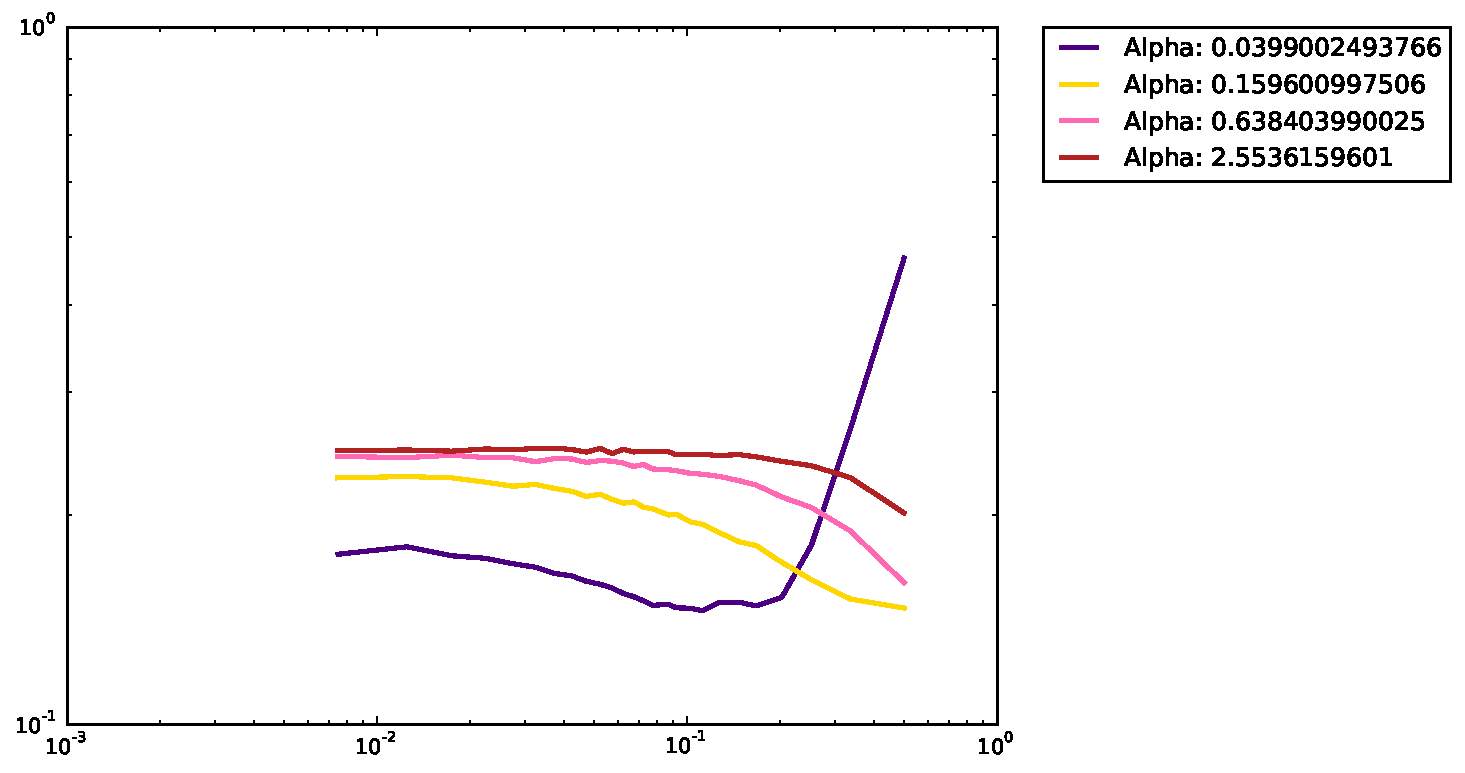
\includegraphics[scale=0.4]{images/results/vicinity_sliding_n401_rounds10000_partial.pdf}
\caption{Plot of normalized variance versus control parameter $\beta$ for various values of $\alpha$  for sliding window one-dimensional communities}
\label{fig:sliding vicinity partial}
\end{center}
\end{figure}

The results are more evident when we look at the values of $\beta$ that minimize the volatility of the model in Table \ref{table:sliding m4}.
While for $\alpha=0.03990025$ we found the optimal value $\beta\approx 0.05$ when isolated communities were used, we have found for the same value of $\alpha$ that $\beta\approx 0.10$ should be used for sliding window communities.
This means that instead of dividing the set of agents in $20$ communities a more realistic partition number should be $10$.
For $\alpha=0.159601$ we can see that the optimal value of $\beta$ is $0.5$ that tells us communities should be larger as we increment $\alpha$ when sliding window communities are concerned.

\begin{table}
\tiny
\centering
\resizebox{\columnwidth}{!}{%
\begin{tabular}{lllllll}
\toprule
neighs &  M &    N &       alpha &         beta & meanNormVar &       var \\
\midrule
    45 &  4 &  401 &  0.03990025 &    0.1122195 &   0.1456658 &  58.41198 \\
    41 &  4 &  401 &  0.03990025 &    0.1022444 &   0.1468764 &  58.89743 \\
    37 &  4 &  401 &  0.03990025 &   0.09226933 &   0.1470761 &  58.97754 \\
    67 &  4 &  401 &  0.03990025 &    0.1670823 &   0.1480023 &  59.34892 \\
    31 &  4 &  401 &  0.03990025 &   0.07730673 &   0.1482901 &  59.46434 \\
\midrule
   201 &  6 &  401 &  0.159601 &    0.5012469 &   0.1469697 &  58.93485 \\
   135 &  6 &  401 &  0.159601 &    0.3366584 &   0.1513832 &  60.70467 \\
   101 &  6 &  401 &  0.159601 &    0.2518703 &   0.1613675 &  64.70837 \\
    81 &  6 &  401 &  0.159601 &     0.201995 &   0.1709139 &  68.53649 \\
    67 &  6 &  401 &  0.159601 &    0.1670823 &   0.1806012 &  72.42107 \\
\bottomrule
\end{tabular}%
}
\caption{Sliding window neighbourhood table}
\label{table:sliding m4}
\end{table}

\subsection{Sliding window von Neumann neighbourhood}

As long as von Neumann vicinity is concerned the results are similar to the first two cases, as expected.
In Figure \ref{fig:von neumann vicinity partial} different curves for different $\alpha$ values are drawn.
Von Neumann neighbourhood is defined only by the radius parameter $R$, so the number of neighbouring agents is reduced to a small subset of all possible natural numbers.
This has led us to the conclusion that von Neumann neighbourhood is not a good candidate to construct links between agents in the case studied.

\begin{figure}[h]
\begin{center}
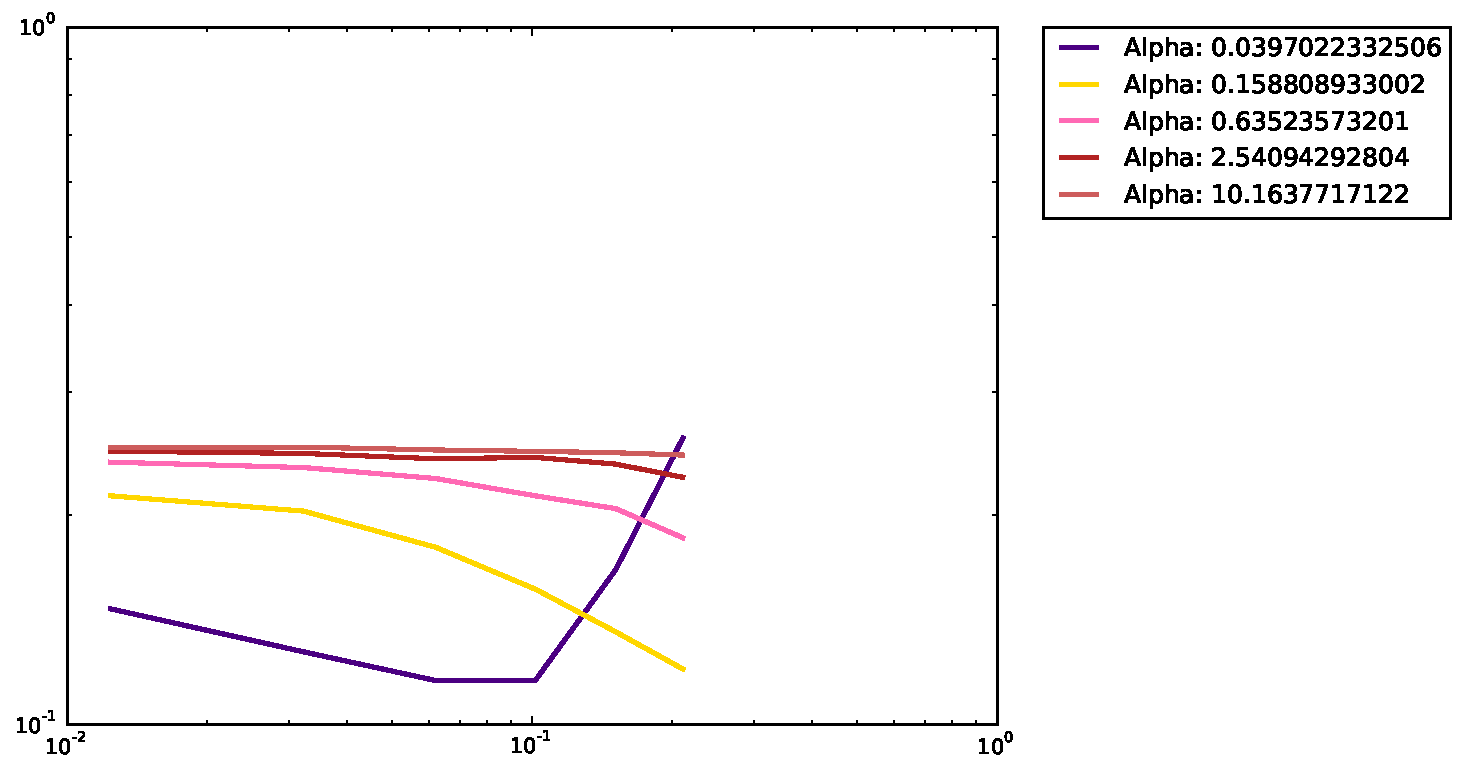
\includegraphics[scale=0.4]{images/results/vicinity_vonNeumann_n403_rounds10000_partial.pdf}
\caption{Plot of normalized variance versus control parameter $\beta$ for various values of $\alpha$  for sliding window two-dimensional communities with von Neumann vicinities}
\label{fig:von neumann vicinity partial}
\end{center}
\end{figure}

In Table \ref{table:vonNeumann table} we show the optimal values of $\beta$ for various values of $\alpha$.
Results are much alike other results for fixed neighbourhoods, for small values of $\alpha$, $\beta$ is in the interval $[0.03,0.12]$, dividing the set of agents into smaller communities.

For higher $\alpha$ values, as we can see in the case of $\alpha=0.6352357$ larger communities are preferred, but if we look ate the values of volatility, ie. mean normalized variance, we can find that the difference between them is small when compared to lower $\alpha$ values. 
This fact can be easily seen in most of the figures, as we increment the $\alpha$ the curves become horizontal lines, telling us that the dimension of the vicinity does not influence greatly the volatility of the game.

\begin{table}
\tiny
\centering
\resizebox{\columnwidth}{!}{%
\begin{tabular}{lllllll}
\toprule
neighs &  M &    N &      alpha &        beta & meanNormVar &       var \\
\midrule
    25 &  4 &  403 &  0.03970223 &  0.06203474 &    0.115673 &  46.61621 \\
    41 &  4 &  403 &  0.03970223 &    0.101737 &   0.1158334 &  46.68086 \\
    13 &  4 &  403 &  0.03970223 &  0.03225806 &   0.1271843 &  51.25529 \\
     5 &  4 &  403 &  0.03970223 &  0.01240695 &     0.14656 &  59.06369 \\
    61 &  4 &  403 &  0.03970223 &   0.1513648 &   0.1668666 &  67.24726 \\
    85 &  4 &  403 &  0.03970223 &   0.2109181 &   0.2574937 &  103.7699 \\
\midrule
    85 &  6 &  403 &  0.1588089 &   0.2109181 &   0.1201926 &  48.43763 \\
    61 &  6 &  403 &  0.1588089 &   0.1513648 &   0.1358312 &  54.73998 \\
    41 &  6 &  403 &  0.1588089 &    0.101737 &   0.1563717 &  63.01779 \\
    25 &  6 &  403 &  0.1588089 &  0.06203474 &   0.1796163 &  72.38538 \\
    13 &  6 &  403 &  0.1588089 &  0.03225806 &   0.2023782 &  81.55843 \\
     5 &  6 &  403 &  0.1588089 &  0.01240695 &   0.2128725 &  85.78764 \\
\midrule
    85 &  8 &  403 &  0.6352357 &   0.2109181 &   0.1853413 &  74.69255 \\
    61 &  8 &  403 &  0.6352357 &   0.1513648 &   0.2040382 &  82.22741 \\
    41 &  8 &  403 &  0.6352357 &    0.101737 &   0.2128382 &  85.77379 \\
    25 &  8 &  403 &  0.6352357 &  0.06203474 &   0.2253677 &  90.82317 \\
    13 &  8 &  403 &  0.6352357 &  0.03225806 &   0.2336805 &  94.17324 \\
     5 &  8 &  403 &  0.6352357 &  0.01240695 &   0.2378988 &  95.87322 \\
\bottomrule
\end{tabular}%
}
\caption{von Neumann neighbourhood}
\label{table:vonNeumann table}
\end{table}

\section{Variable community structures results}
\label{sec:hierarchical}

Fixed communities are easy to implement and optimize, yet they are not representative of real world examples.
Different network topologies have been introduced in Sections \ref{sec:scale free}, \ref{sec:small world} and \ref{sec:hierarchical vicinity}. Here we report the experimental results of those network structures.

\subsection{Scale free results}

Scale free networks generated with Barabasi-Albert algorithm create one large community in which different nodes have different degrees, based on their popularity.
By using the peripheral attachment mechanism some nodes end up with greater neighbourhoods while the last nodes that are added belong to smaller communities.

\begin{figure}[h]
\begin{center}
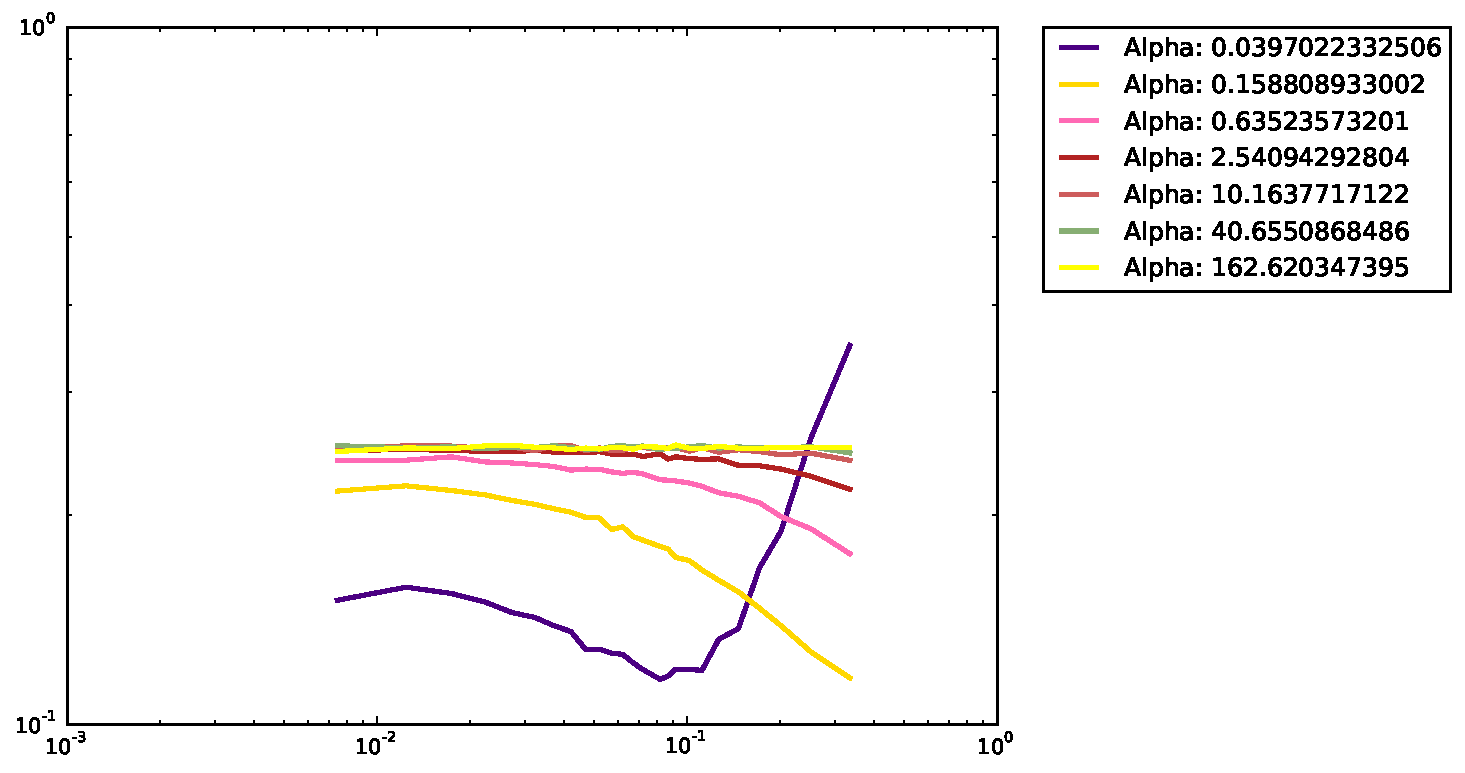
\includegraphics[scale=0.4]{images/results/vicinity_Barabasi_n403_rounds10000_partial.pdf}
\caption{Plot of normalized variance versus control parameter $\beta$ for various values of $\alpha$  for scale free communities generated with Barabasi-Albert algorithm}
\label{fig:scale free vicinity partial}
\end{center}
\end{figure}

As long as the number of edges a nodes in the graph is considered, we have calculated the mean degree of nodes for scale free networks, and use that number to calculate a mean $\beta$ value.
Results are show in Table \ref{table:Scale free vicinity table}, from which we can see that scale free topology performs consistently better than pure sliding window vicinity structure and a little better than von Neumann neighbourhood.
On the other hand it is worse off than patch network, and this result is not surprising as we have already theorized on the better performance of patch network due to its isolated communities.

Optimal value for scale free network for $\beta$ is in the interval $[0.13,0.19]$ for $\alpha=0.03970223$ while it is significantly higher for $\alpha=0.1588089$ and is close to $0.5$.
Note that in the column \textit{neighs} we show the mean degree of nodes, and not the parameter $k$ used to generate the scale free network with the Barabasi-Albert algorithm.
The parameter $k$ tells us to how many nodes a newcomer should be connected, hence the mean degree of nodes will be higher unless we start with an already built structure.
For example to obtain an average $61$ neighbouring nodes as is optimal for $\alpha=0.03970223$ we should use $k=33$ and so on.

\begin{table}
\tiny
\centering
\resizebox{\columnwidth}{!}{%
\begin{tabular}{lllllll}
\toprule
neighs &  M &    N &       alpha &        beta & meanNormVar &       var \\
\midrule
    61 &  4 &  403 &  0.03970223 &   0.1513648 &   0.1161257 &  46.79867 \\
    64 &  4 &  403 &  0.03970223 &   0.1588089 &   0.1173796 &  47.30398 \\
    80 &  4 &  403 &  0.03970223 &   0.1985112 &   0.1196375 &  48.21391 \\
    74 &  4 &  403 &  0.03970223 &   0.1836228 &    0.120003 &  48.36119 \\
    54 &  4 &  403 &  0.03970223 &    0.133995 &   0.1200037 &  48.36148 \\
\midrule
   180 &  6 &  403 &  0.1588089 &   0.4466501 &   0.1166436 &  47.00736 \\
   151 &  6 &  403 &  0.1588089 &   0.3746898 &   0.1271984 &  51.26096 \\
   129 &  6 &  403 &  0.1588089 &   0.3200993 &   0.1386061 &  55.85824 \\
   114 &  6 &  403 &  0.1588089 &   0.2828784 &   0.1468814 &  59.19321 \\
   101 &  6 &  403 &  0.1588089 &   0.2506203 &   0.1550459 &  62.48349 \\
\bottomrule
\end{tabular}%
}
\caption{Scale free neighbourhood table}
\label{table:Scale free vicinity table}
\end{table}

\subsection{Small world results}

Results for small world are shown in Figure \ref{fig:small world vicinity partial} and numerical results can be found in Table \ref{table:Small world vicinity table}.
We can see that when the value of the volatility is concerned, there are no significant changes from scale free case, however the optimal values of $\beta$ are different.
In this case the degree of a node is same for all the nodes in the network, as edges are just rewired, not added nor deleted.
Optimal values for $\beta$ are in the interval $[0.8,0.11]$ for $\alpha=0.03970223$, while for $\alpha=0.1588089$ it is preferable to have a higher value of $\beta$ as in other cases.

\begin{figure}[h]
\begin{center}
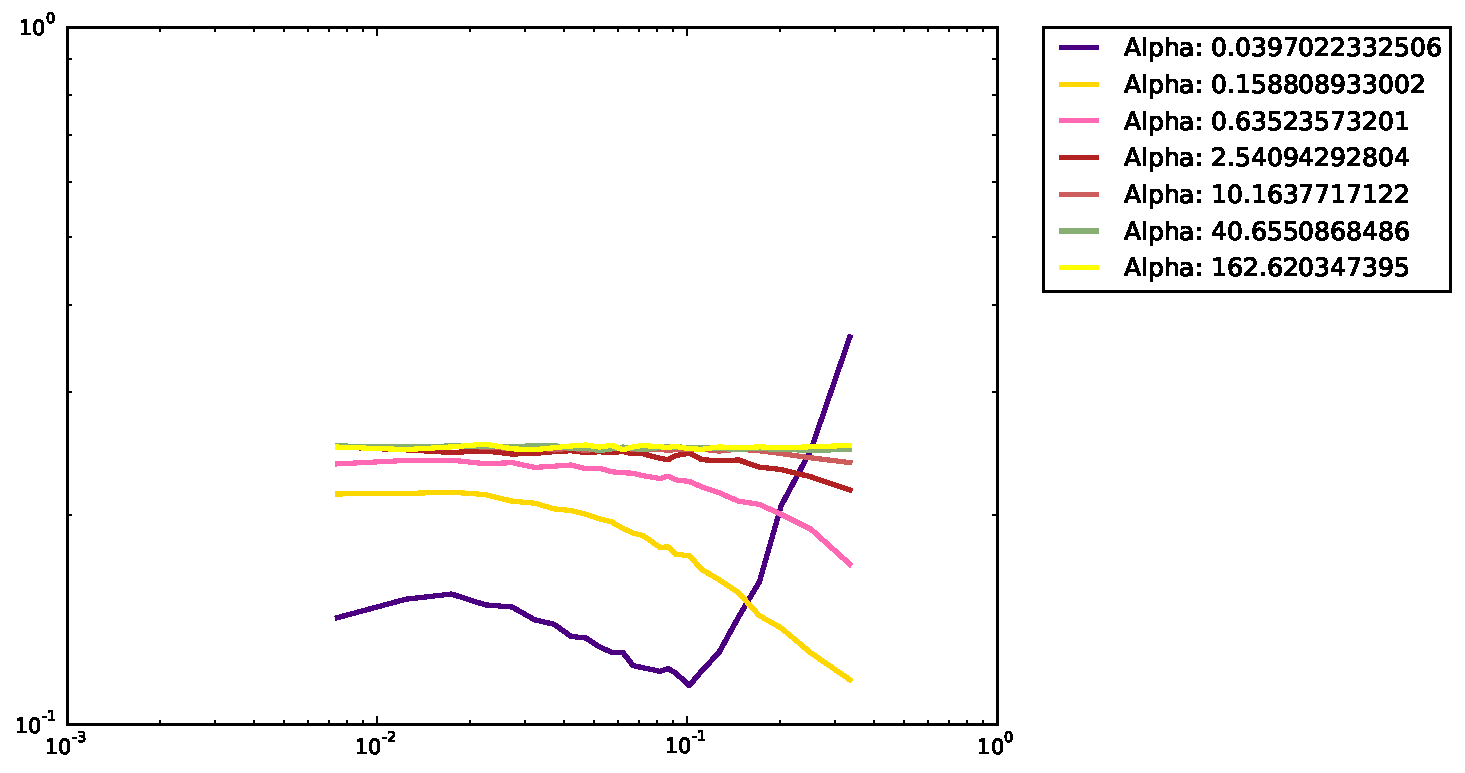
\includegraphics[scale=0.4]{images/results/vicinity_WattsStrogatz_n403_rounds10000_partial.pdf}
\caption{Plot of normalized variance versus control parameter $\beta$ for various values of $\alpha$  for small world communities generated with Watts-Strogatz algorithm}
\label{fig:small world vicinity partial}
\end{center}
\end{figure}

\begin{table}
\tiny
\centering
\resizebox{\columnwidth}{!}{%
\begin{tabular}{lllllll}
\toprule
neighs &  M &    N &       alpha &         beta & meanNormVar &       var \\
\midrule
    41 &  4 &  403 &  0.03970223 &     0.101737 &   0.1138109 &   45.8658 \\
    37 &  4 &  403 &  0.03970223 &   0.09181141 &   0.1185464 &  47.77421 \\
    33 &  4 &  403 &  0.03970223 &   0.08188586 &   0.1192244 &  48.04742 \\
    45 &  4 &  403 &  0.03970223 &    0.1116625 &   0.1195567 &  48.18135 \\
    35 &  4 &  403 &  0.03970223 &   0.08684864 &   0.1203266 &  48.49161 \\
\midrule
   135 &  6 &  403 &  0.1588089 &    0.3349876 &   0.1159726 &  46.73697 \\
   101 &  6 &  403 &  0.1588089 &    0.2506203 &   0.1267708 &  51.08865 \\
    81 &  6 &  403 &  0.1588089 &    0.2009926 &   0.1376265 &  55.46349 \\
    69 &  6 &  403 &  0.1588089 &    0.1712159 &   0.1432754 &  57.73999 \\
    59 &  6 &  403 &  0.1588089 &     0.146402 &   0.1546167 &  62.31052 \\
\bottomrule
\end{tabular}%
}
\caption{Small world neighbourhood}
\label{table:Small world vicinity table}
\end{table}

%\subsection{Hierarchical network results}

%\begin{figure}[h]
%\begin{center}
%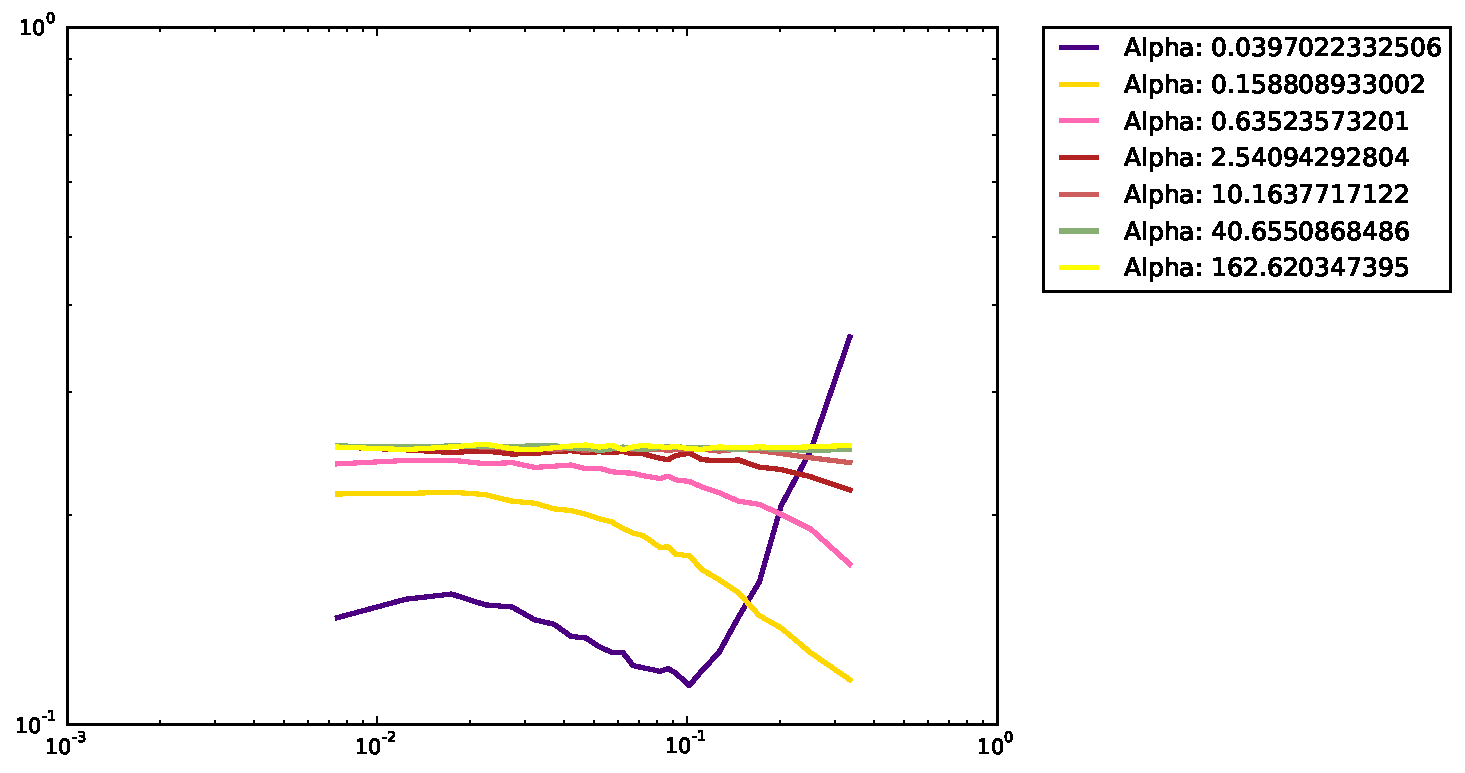
\includegraphics[scale=0.4]{images/results/vicinity_WattsStrogatz_n403_rounds10000_partial.pdf}
%\caption{Plot of normalized variance versus control parameter $\beta$ for various values of $\alpha$  for small world communities generated with Watts-Strogatz algorithm}
%\label{fig:scale free vicinity partial}
%\end{center}
%\end{figure}

%\begin{table}
%\tiny
%\centering
%\resizebox{\columnwidth}{!}{%
%%
%}
%\caption{von Neumann neighbourhood}
%\label{table:vonNeumann table}
%\end{table}

\section{Confrontation of different topologies}
\label{sec:confrontation}

After examining first results we can see that community structure does influence the efficiency of the model, but we have to understand does it do better than basic minority game.
It is easy to see that a model where agents have $M$ bits available for local history and $M$ bits available for global history will outperform a basic agent that has $M$ bit for only global history.
This is true as long as $\alpha$ is kept lower or slightly above its critical value.
But how does our \textit{community} agent bode against a basic agent with $2M$ bits to process global history?
In this case the quantity of information available to both agents is the same, $2M$ bits, but the quality of information is different.
Is our intuition to differentiate information in spatial and temporal justified?

In Figure \ref{fig:fixed vicinity full classic} we show plot the volatility of the model versus the $\beta$ parameter introduced as the percentage of neighbours to total number of agents.
In full lines is shown the volatility of models with community agents, while in the dotted line one can see the volatility of a basic minority game for the same $\alpha$ value.
As we can easily see, for fixed patch neighbourhoods, the introduction of spatial information in the form of communities renders the model more efficient in terms of resource distribution.
The basic minority games performs better only when high values of $\beta$ are used, which means that communities become so large that they start overlapping with global set and hence information is duplicated.

\begin{figure}[h]
\begin{center}
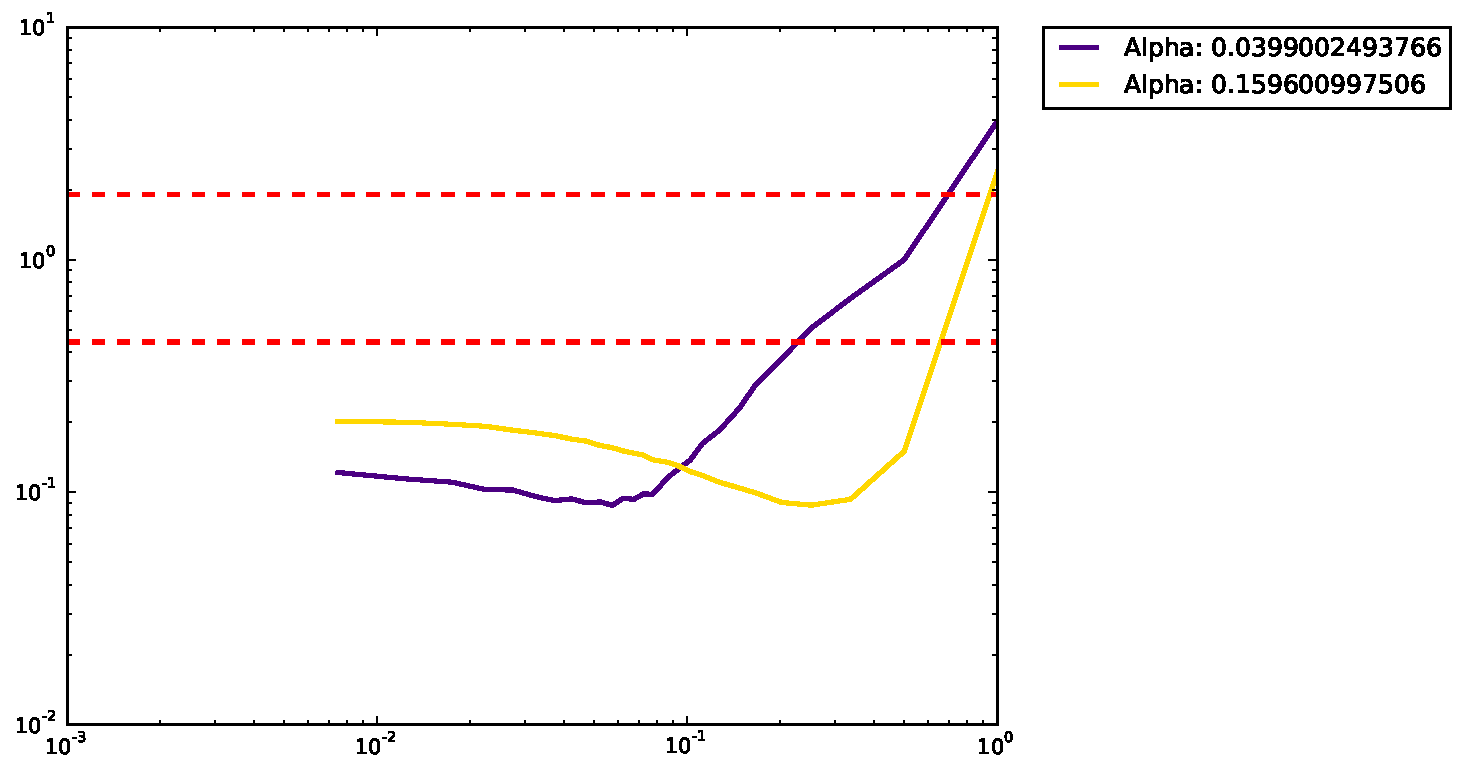
\includegraphics[scale=0.4]{images/results/vicinity_patch_n401_rounds10000_full_time.pdf}
\caption{MGs with fixed patch vicinity in full line vs classic minority game in dotted line for different $\alpha$ values}
\label{fig:fixed vicinity full classic}
\end{center}
\end{figure}

The confrontation between different topologies shed other light on the problem.
In Figure \ref{fig:topologies confrontation 2} we confront different network structures for $\alpha=0.03970223$.
These curves have already been plotted separately as results of each topology, but when we plot them together we can arrive to certain conclusions.
The fixed patch topology, with its isolated communities, is the optimal one.
Fixed patch topology gives us the lowest volatility in a model while also organizing our set into smaller communities.
We already theorized that by separating agents into communities that don't exchange information should make the model more efficient, and it has been confirmed by these experimental results.
On the other hand sliding window topology has the worst performance as it has a complementary philosophy with respect to fixed patch one.
While in the first case agents that are neighbours by definition belong to the same community, in sliding window topology no two agents belong to the same community as it is defined ad hoc per agent.
This makes the exploitation of information much more difficult, and as a result leaves the model with higher volatility and larger communities in its best case scenario.

The scale free and small world topologies are the middle ground.
They are generated randomly to some extent, in scale free case we have peripheral attachment that is the probability to be assigned to certain communities, and in small world case we have the rewiring that perturbs the graph edges.
In this way these \textit{real world} topologies retain the free flow of information between communities, and yet have a chance to isolate them more between each other when compared to sliding window technique.

In Figure \ref{fig:topologies confrontation 3} we show same kind of results for different topologies for a different value of $\alpha=0.1588089$.
As we can see the optimal values of $\beta$ change, but qualitatively the results remain the same.
After we have passed the critical value of $\alpha$ the community structure seems to worsen the efficiency of the model, but this consideration does not take into account the \textit{credibility} of information.
This point will be tackled in Chapter \ref{chapter:algorithm}.

\begin{figure}[h]
\begin{center}
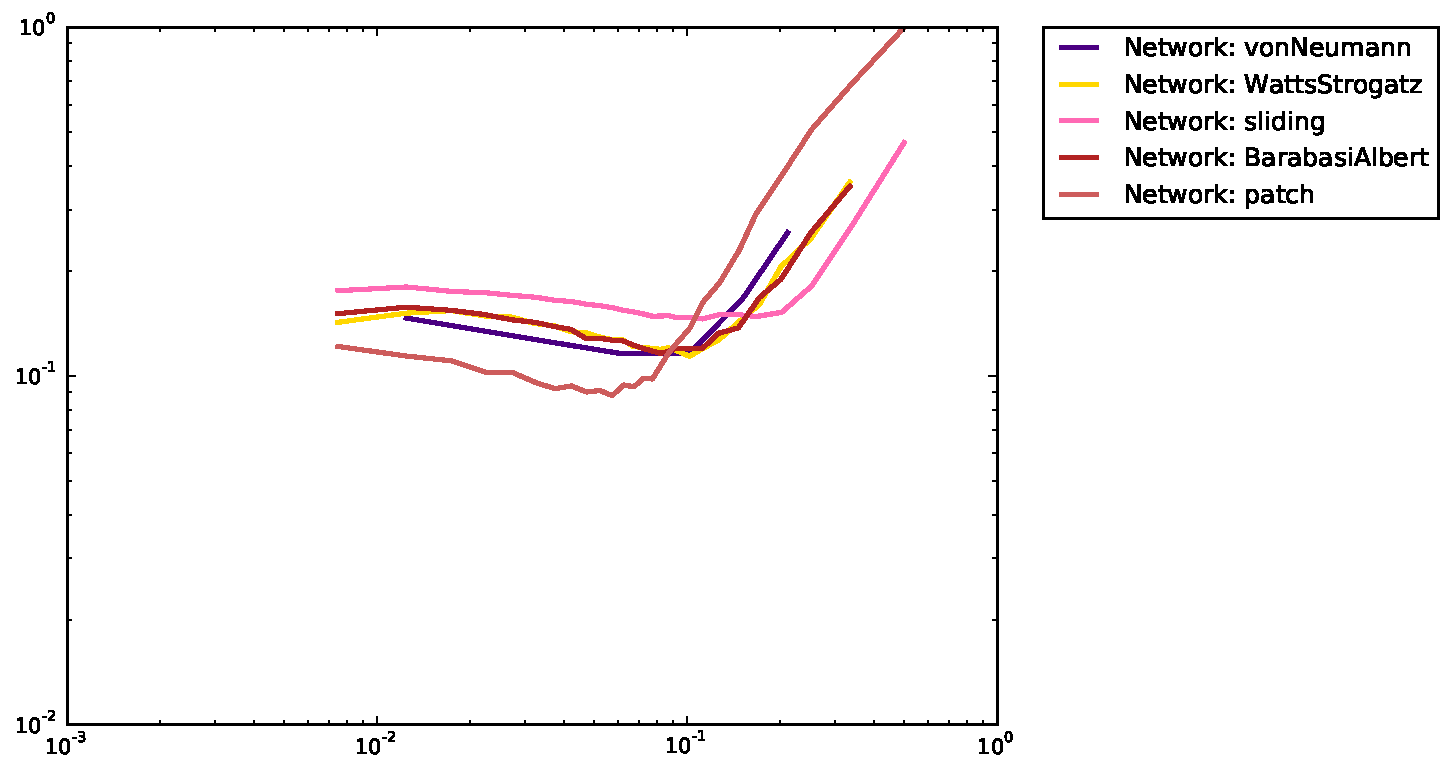
\includegraphics[scale=0.4]{images/results/topologies_confront_m2.pdf}
\caption{Different topologies confrontation. Percentage of neighbouring agents on x axis, volatility on y axis, and 2 bits to local MG and 2 bits to global MG}
\label{fig:topologies confrontation 2}
\end{center}
\end{figure}

\begin{figure}[h]
\begin{center}
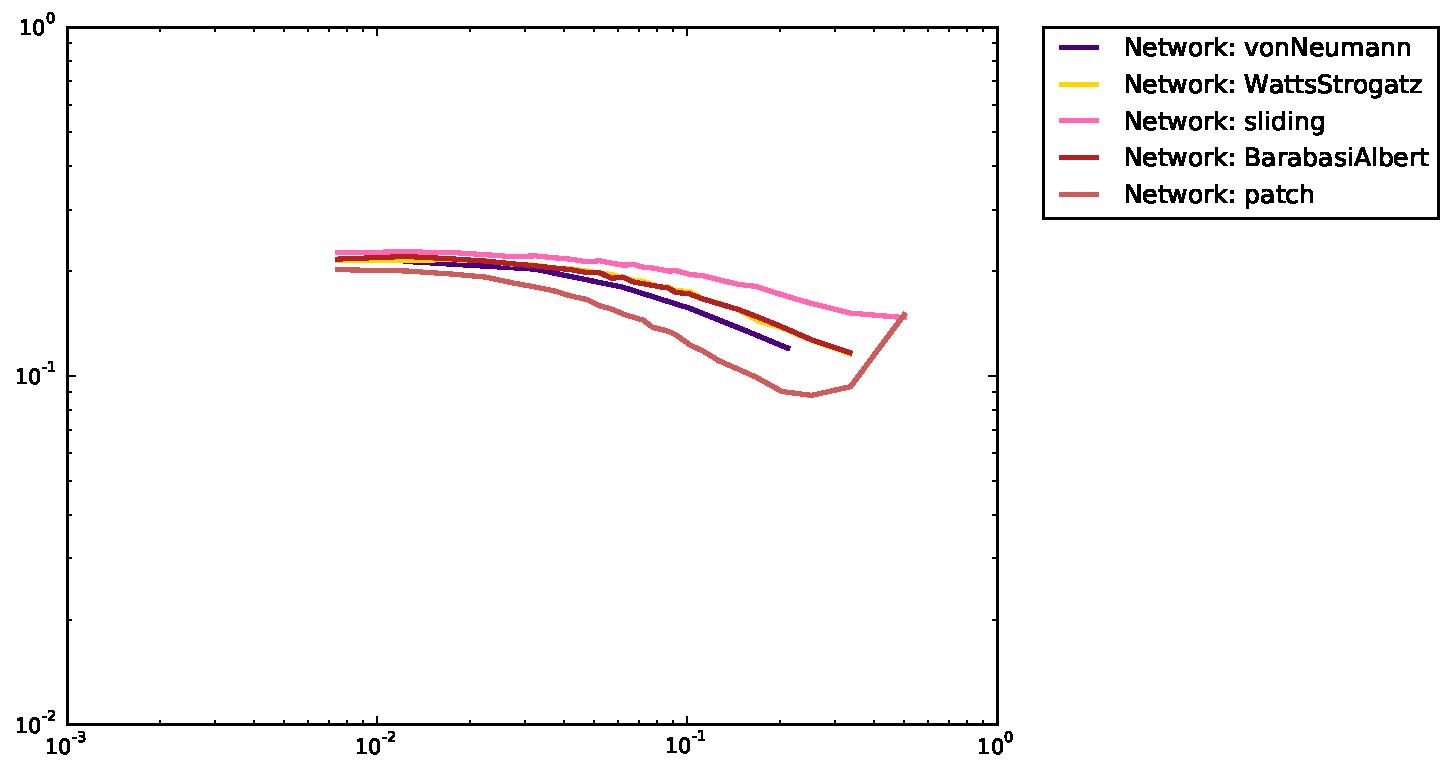
\includegraphics[scale=0.4]{images/results/topologies_confront_m3.pdf}
\caption{Different topologies confrontation. Percentage of neighbouring agents on x axis, volatility on y axis, and 3 bits to local MG and 3 bits to global MG}
\label{fig:topologies confrontation 3}
\end{center}
\end{figure}
% Conclusions
\chapter{Conclusions}
\label{chapter:conclusions}


\phantomsection
\addcontentsline{toc}{chapter}{Bibliography}
\bibliographystyle{unsrt}
\bibliography{bibliography}
\end{document}
